\documentclass[article, 12pt, 3p]{elsarticle}

\usepackage{natbib} 
\setcitestyle{authoryear,open={(},close={)}}
%\bibliographystyle{plainnat}

\usepackage{etoolbox,comment,setspace,fancyhdr,hyperref,color,graphicx,subcaption,booktabs,rotating,multirow}

\captionsetup[subfigure]{labelformat=simple,labelsep=space}
\renewcommand\thesubfigure{(\roman{subfigure})}

\newcounter{rowfig}
\renewcommand{\therowfig}{\Alph{rowfig}}

\usepackage{amsmath,amsthm,amssymb,amstext,bbold,amsfonts}
\usepackage{float,caption}
\usepackage{threeparttable}
\usepackage{lscape}
\usepackage{bbm}
\usepackage{adjustbox}
\usepackage[tracking=true]{microtype}
%\usepackage[pdftex, letterpaper, margin=1in, headheight=-.25cm]{geometry}
 %\usepackage[abbr]{harvard}
 
\hypersetup{
  colorlinks   = true, %Colours links instead of ug dly boxes
  urlcolor     = blue, %Colour for external hyperlinks
  linkcolor    = black, %Colour of internal links 
  citecolor   = blue %Colour of citations
}

\newtheorem{proposition}{Proposition}
\newtheorem{definition}{Definition}
\newtheorem{assumption}{Assumption}
\newtheorem{condition}{Condition}
\newtheorem{lemma}{Lemma}
\newtheorem{conjecture}{Conjecture}
\newtheorem{corollary}{Corollary}
\numberwithin{corollary}{proposition}
%\numberwithin{equation}{section}
% [[prompt01]] original: \numberwithin{equation}{}

%\newcommand{\inv}{\makebox[0pt][l]{$^{-1}$}}
\pdfoptionpdfminorversion=6 

%Define argmax
\DeclareMathOperator*{\argmax}{arg\,max}

%%Put space between captions and figures.
%\setlength{\belowcaptionskip}{6pt}

\makeatletter
\def\ps@pprintTitle{%
   \let\@oddhead\@empty
   \let\@evenhead\@empty
   \let\@oddfoot\@empty
   \let\@evenfoot\@oddfoot
}
\makeatother
\usepackage{ragged2e}
\usepackage{setspace} 
\usepackage{caption}
% [[prompt01]] original: \usepackage[usenames,dvipsnames]{pstricks}
% [[prompt01]] original: \usepackage{epsfig}
% [[prompt01]] original: \usepackage{pst-grad} % For gradients
% [[prompt01]] original: \usepackage{pst-plot} % For axes
 \usepackage[space]{grffile} % For spaces in paths
 \makeatletter % For spaces in paths
 \patchcmd\Gread@eps{\@inputcheck#1 }{\@inputcheck"#1"\relax}{}{}
 \makeatother
\usepackage[utf8]{inputenc}
% [[prompt01]] original: \usepackage{stackrel}
\IfFileExists{stackrel.sty}{\usepackage{stackrel}}{}
\usepackage{array}
\usepackage{siunitx}
% [[prompt02]] added: column-width convention of the reference (_reference_productivity/Tables/_tabledefs.tex,
% copied, not \input): N{<width>} centred numeric column, L{<width>} ragged-right label column.
\usepackage{makecell}
\newcolumntype{N}[1]{>{\centering\arraybackslash}p{#1}}
\newcolumntype{L}[1]{>{\raggedright\arraybackslash}p{#1}}
\newlength{\labelw}\setlength{\labelw}{0.22\textwidth}
\newlength{\labelwwide}\setlength{\labelwwide}{0.36\textwidth}
\newlength{\labelwnarrow}\setlength{\labelwnarrow}{0.19\textwidth}
\newcommand{\colwfor}[2]{\dimexpr(\textwidth-(#2)-\tabcolsep*\numexpr2*#1+2\relax)/#1\relax}
\newcommand{\colwform}[3]{\dimexpr(\textwidth-(#3)-\tabcolsep*\numexpr2*#1+2*#2\relax)/#1\relax}
\newcommand{\colw}{\colwfor{6}{\labelw}}
\newcommand{\colwvii}{\colwfor{7}{\labelw}}
\newcommand{\colwnarrow}{\colwfor{8}{\labelw}}
\newcommand{\notesize}{\footnotesize}
\setlength{\extrarowheight}{4pt}
\renewcommand\normalsize{\fontsize{11}{8}\selectfont}
\newcommand\narrowstyle{\SetTracking{encoding=*}{-10}\lsstyle}
\newcommand\vnarrowstyle{\SetTracking{encoding=*}{-40}\lsstyle}
\newcommand\vvnarrowstyle{\SetTracking{encoding=*}{-75}\lsstyle}

\newcommand\narrowtext[1]{\textls[-10]{#1}}
\newcommand\vnarrowtext[1]{\textls[-40]{#1}}
\newcommand\vvnarrowtext[1]{\textls[-75]{#1}}

\makeatletter
\renewcommand\footnotesize{%
   \@setfontsize\footnotesize\@ixpt{9}%
   \abovedisplayskip 8\p@ \@plus2\p@ \@minus4\p@
   \abovedisplayshortskip \z@ \@plus\p@
   \belowdisplayshortskip 4\p@ \@plus2\p@ \@minus2\p@
   \def\@listi{\leftmargin\leftmargini
               \topsep 4\p@ \@plus2\p@ \@minus2\p@
               \parsep 2\p@ \@plus\p@ \@minus\p@
               \itemsep \parsep}%
   \belowdisplayskip \abovedisplayskip
}
\makeatother

\usepackage{setspace}
\usepackage[T1]{fontenc}
\usepackage{lmodern}  % [[v3]] scalable fonts, needed by microtype outside Overleaf
\usepackage{array}
\usepackage{longtable}
\usepackage{pdfpages}
\usepackage{dsfont}
\newcommand{\bc}{\begin{center}}
\newcommand{\ec}{\end{center}}
\newcommand{\bt}{\begin{tabular}}
\newcommand{\et}{\end{tabular}}
\newcommand{\bi}{\begin{itemize}}
\newcommand{\ei}{\end{itemize}}
\newcommand{\ben}{\begin{enumerate}}
\newcommand{\een}{\end{enumerate}}
\newcommand{\bd}{\begin{displaymath}}
\newcommand{\ed}{\end{displaymath}}
\newcommand{\beann}{\begin{eqnarray*}}
\newcommand{\eeann}{\end{eqnarray*}}
\newcommand{\bea}{\begin{eqnarray}}
\newcommand{\eea}{\end{eqnarray}}
\newcommand{\ba}{\begin{array}}
\newcommand{\ea}{\end{array}}
\newcommand{\bma}{\begin{pmatrix}}
\newcommand{\ema}{\end{pmatrix}}
%}}}
%Math Shortcuts {{{
\newcommand{\Ra}{\Rightarrow}
\newcommand{\bbR}{\mathbb{R}}
\newcommand{\bbY}{\mathbb{Y}}
\newcommand{\bbF}{\mathbb{F}}
\newcommand{\bbS}{\mathbb{S}}
\newcommand{\bbN}{\mathbb{N}}
\newcommand{\bbG}{\mathbb{G}}
\newcommand{\bbT}{\mathbb{T}}
\newcommand{\deB}{\mathcal{B}}
\newcommand{\deW}{\mathcal{W}}
\newcommand{\deR}{\mathcal{R}}
\newcommand{\deF}{\mathcal{F}}
\newcommand{\deA}{\mathcal{A}}
\newcommand{\deY}{\mathcal{Y}}
\newcommand{\deS}{\mathcal{S}}
\newcommand{\deL}{\mathcal{L}}
\newcommand{\deH}{\mathcal{H}}
\newcommand{\deE}{\mathcal{E}}
\newcommand{\deP}{\mathcal{P}}
\newcommand{\deG}{\mathcal{G}}
\newcommand{\deT}{\mathcal{T}}
\newcommand{\deff}{\mathcal{f}}
\newcommand{\dep}{\mathcal{p}}
\newcommand{\E}{\mathnormal{E}}
\newcommand{\var}{\mathnormal{V\!AR}}
\newcommand{\Cov}{\mathnormal{COV}}
\newcommand{\Corr}{\mathnormal{CORR}}
\newcommand{\Prob}{\mathnormal{Prob}}
%}}}
%Additional Shortcuts {{{
\newcommand{\mD}{\displaystyle}
\newcommand{\mT}{\textstyle}
\newcommand{\mS}{\scriptstyle}
\newcommand{\mSS}{\scriptscriptstyle}
\newcommand{\m}[1]{\,#1\,}
\newcommand{\nn}{\nonumber}
\newcommand{\colorEmphText}{\color{blue}}
\newcommand{\colorEmphBackground}{\color{yellow}}
%}}}
% \usepackage[stable]{footmisc} 
\newcommand*{\mycommand}[1]{\texttt{\emph{#1}}}
% [[prompt01]] original: \renewcommand*{\thefootnote}{\fnsymbol{footnote}}
%% these three are essential for estout
\usepackage{booktabs}  % neatly formatting lines
\usepackage{threeparttable}    
\usepackage{dcolumn}    % aligning decimals
    \newcolumntype{d}[1]{D{.}{.}{#1}}
% Estout LaTeX wrapper (by Jörg Weber)
\let\estinput=\input % define a new input command so that we can still flatten the document
\newcommand{\estwide}[3]{
		\vspace{.75ex}{
			%\textsymbols% Note the added command here
			\begin{tabular*}
			{\textwidth}{@{\hskip\tabcolsep\extracolsep\fill}l*{#2}{#3}}
			\toprule
			\estinput{#1}
			\addlinespace[.75ex]
			\end{tabular*}
			}
		}	
\newcommand{\estauto}[3]{
		\vspace{.75ex}{
			%\textsymbols% Note the added command here
			\begin{tabular}{l*{#2}{#3}}
			\toprule
			\estinput{#1}
			\\ \bottomrule           % 08 Dec 2021. Add these slashes.
			\addlinespace[-.75]
			\end{tabular}
			}
		}
% Allow line breaks with \\ in specialcells
\newcommand{\specialcell}[2][c]{%
    \begin{tabular}[#1]{@{}c@{}}#2\end{tabular}
}
\usepackage{float}
\usepackage[section]{placeins}
% [[prompt02d]] floats share pages with text instead of going to float pages
\renewcommand{\topfraction}{0.9}
\renewcommand{\bottomfraction}{0.8}
\renewcommand{\textfraction}{0.07}
\renewcommand{\floatpagefraction}{0.85}
\setcounter{topnumber}{3}
\setcounter{bottomnumber}{2}
\setcounter{totalnumber}{4}
\setlength{\floatsep}{10pt plus 2pt minus 2pt}
\setlength{\textfloatsep}{14pt plus 2pt minus 2pt}
\setlength{\intextsep}{12pt plus 2pt minus 2pt}
\newcommand{\sym}[1]{\rlap{#1}}% Thanks David Carlisle
\usepackage{hhline}
\captionsetup{font=normalsize} 


 % Note/Source/Text after Tables
\newcommand{\figtext}[1]{
	\vspace{-1.9ex}
	\captionsetup{justification=justified,font=scriptsize}
	\caption*{\hspace{6pt}\hangindent=1.5em #1}
	} 
\newcommand{\fignote}[1]{\figtext{\emph{Note:~}~#1}}

\newcommand{\figsource}[1]{\figtext{\emph{Source:~}~#1}}

% Add significance note with \starnote
\newcommand{\starnote}{\figtext{* p < 0.1, ** p < 0.05, *** p < 0.01. Standard errors in parentheses.}}
% [[prompt01]] added: source note of every table and figure (wording from main.tex l. 16)
% [[prompt02]] original: \newcommand{\srcnote}{\textit{Source:} Authors' calculations based on customs data matched to Orbis and Dun \& Bradstreet.}
\newcommand{\srcnote}{\textit{Source:} Authors' calculations based on customs data matched to Orbis (Bureau van Dijk) and Dun \& Bradstreet.}
%\usepackage{etoolbox} % to hook into `figure` and reset the mysubfig counter

% [[prompt01]] original: \usepackage{subfig}


% Checkmarks
\usepackage{tikz}
\newcommand{\tikzxmark}{%
\tikz[scale=0.23] {
    \draw[line width=0.7,line cap=round] (0,0) to [bend left=6] (1,1);
    \draw[line width=0.7,line cap=round] (0.2,0.95) to [bend right=3] (0.8,0.05);
}}
\newcommand{\tikzcmark}{% 
\tikz[scale=0.23] {
    \draw[line width=0.7,line cap=round] (0.25,0) to [bend left=10] (1,1);
    \draw[line width=0.8,line cap=round] (0,0.35) to [bend right=1] (0.23,0);
}}
%\renewcommand{\arraystretch}{0.9}
% [[prompt02]] original: \renewcommand{\arraystretch}{0.8}
% [[prompt02]] original: \setlength{\tabcolsep}{5pt}
 \makeatletter
\newcommand*\mysize{%
  \@setfontsize\mysize{7.5}{9.0}%
}

\makeatother
% For reference:
%\[
%    \checkmark
%    \tikzxmark
%    \tikzcmark
%\]

%\onehalfspacing

% [[prompt03b]] elsarticle draws two rules around the (absent) abstract; suppress them for this summary
\makeatletter
\let\els@maketitle\maketitle
\renewcommand{\maketitle}{\begingroup\let\hrule\relax\els@maketitle\endgroup}
\makeatother
\hyphenpenalty=10000 \exhyphenpenalty=10000  % [[v3]] no words split across lines with a hyphen
\begin{document}

\title{$\,$\\ $\,$\\ $\,$\\\vspace{-4.9em}\LARGE\textbf{Multinational Firms and Agricultural Trade in Latin America}\footnote{The views and interpretations in this paper are strictly those of the authors and should not be attributed to the Inter-American Development Bank, its executive directors, or its member countries.}}
\author{\vskip 2em This version: November 2026\\[2pt] \small Preliminary draft, please do not circulate}

\thispagestyle{empty}
\maketitle
\setcounter{page}{0}\setcounter{footnote}{0}
\renewcommand\normalsize{\fontsize{12}{20}\selectfont}\normalsize
\newpage

\section{Introduction}\label{sec:intro}

Agriculture accounts for 35 percent of the merchandise exports of the nine Latin American countries studied here,
and for more than half in Argentina, Paraguay and Uruguay. Much of world agricultural trade goes through a few large
firms. Four trading companies handle most of the world grain trade (Murphy, Burch and Clapp, 2012, and Clapp, 2015),
and multinational firms lead the processing, trading and retail stages of agricultural value chains (UNCTAD, 2009,
and Reardon et al., 2009). Yet there is little systematic evidence on how much of the agricultural exports of the
region is shipped by multinational firms, where these firms are based, and how the exports of other firms relate to
their presence.

This note documents these patterns with customs records for all the agricultural exports of nine countries, linked
to ownership data on multinational groups. Agriculture differs from manufacturing in ways that matter for the role of
multinational firms. Some products, such as grains and oilseeds, are grown on large areas with machinery and are
shipped in bulk through storage, crushing and port facilities. Others, such as fruit, vegetables and coffee, depend
on labor at harvest and are grown by many smaller farms. We therefore classify agricultural products by type of
production and by the capital intensity of the industry that produces them, and we compare the presence of
multinationals and its association with exports across these groups. We also look at the products in which
multinationals operate and split the exports of local firms into the number of exporters and the exports per
exporter.

We document six stylized facts. Multinational firms ship almost half of the agricultural exports of the region
(Fact 1). Their parents are based in a few countries (Fact 2), and a few large groups ship most of the exports of
foreign affiliates (Fact 3). Exports are larger where more multinationals export the same product to the same
destination, and so are the exports of local firms (Fact 4). This association is stronger for field crops and for
farm products made with more capital per worker (Fact 5). The exports of multinationals do not fall less with
distance than those of local firms once the same firm is compared across destinations (Fact 6).

Facts 1 to 3 are descriptive. Facts 4 to 6 come from regressions that start with origin, destination, product and
year fixed effects and add stricter fixed effects one step at a time. A workbook that accompanies this note reports
every specification, also those that the tables do not show. These regressions describe associations, not causal
effects. Section~\ref{sec:data} describes the data and the classification of agricultural products.
Section~\ref{sec:facts} presents the stylized facts, first for the nine countries together and then country by
country. Section~\ref{sec:conclusions} concludes.

\section{Data}\label{sec:data}

\subsection{Customs and Ownership Data}

The data come from two sources. The first is the export transactions recorded by the customs agencies of nine Latin
American countries: Argentina, Chile, Colombia, Costa Rica, the Dominican Republic, El Salvador, Paraguay, Peru and
Uruguay. For each export, they report the exporting firm, the product, the destination, the year and the value.
Products are defined at six digits of the Harmonized System (HS), and agricultural products are HS chapters 01 to 24.
The period is 2012 to 2018, the years in which all nine countries are observed. The second source is ownership data
from Orbis, compiled by Bureau van Dijk, and from Dun \& Bradstreet. Both report the global ultimate owner of each
company, that is, the company at the top of its ownership chain, and the country of that owner. Exporters are linked
to these records by tax identifiers, by name matching confirmed with a large language model, and by a manual review
of the largest exporters that remained unmatched. Over 2012 to 2018, the country of the ultimate owner is known for
89 percent of the agricultural exports of foreign affiliates.

An exporter linked to the ownership data is an affiliate of a multinational firm (MNE), and its ultimate owner is its
parent. The affiliate is a domestic MNE when its parent is located in the exporting country and a foreign MNE
otherwise. Exporters that cannot be linked are local firms. A multinational group is the set of affiliates with the
same parent. In 2018, 12,993 firms exported 875 agricultural products to 211 countries, for a total of US\$78.5 billion
(Table~\ref{tab:sample}). The weight of agriculture in merchandise exports varies widely across the nine countries. It
is 84 percent in Paraguay, 56 percent in Argentina and 52 percent in Uruguay, and between 17 and 24 percent in
Colombia, El Salvador, Peru, the Dominican Republic and Chile. Argentina alone ships 44 percent of the agricultural
exports of the region.

% ---- Table: Agricultural exports, by exporting country, 2018
\begin{table}[htbp]
\centering
\caption{Agricultural exports, by exporting country, 2018}
\label{tab:sample}
{\footnotesize\setlength{\tabcolsep}{4pt}\setlength{\extrarowheight}{1pt}
\adjustbox{max width=\linewidth}{\begin{tabular}{lrrrrr}
\toprule
Country & Exporters & Products & Destinations & Exports (US\$ billion) & Agriculture in total exports (\%) \\
\midrule
Argentina & 2,879 & 474 & 176 & 34.6 & 56.3 \\
Peru & 2,538 & 451 & 146 & 10.0 & 20.9 \\
Chile & 1,542 & 452 & 164 & 8.5 & 24.1 \\
Colombia & 2,421 & 448 & 166 & 7.2 & 17.3 \\
Paraguay & 358 & 171 & 113 & 6.6 & 83.8 \\
Costa Rica & 1,123 & 438 & 127 & 4.8 & 42.5 \\
Uruguay & 357 & 193 & 111 & 3.5 & 52.0 \\
Dominican Republic & 1,342 & 483 & 124 & 2.2 & 23.4 \\
El Salvador & 433 & 342 & 82 & 1.1 & 18.8 \\
\midrule
LAC9 & 12,993 & 875 & 211 & 78.5 & 34.5 \\
\bottomrule
\end{tabular}
}}

\begin{minipage}{0.95\linewidth}
\notesize
\vspace{0.6em}
\textit{Notes:} Agricultural exports (HS chapters 01 to 24) in 2018. Exporters are distinct tax identifiers within each country. Destinations are importing countries with an ISO 3166 country code. Free trade zones and shipments to the exporting country itself are not counted. LAC9: the nine countries together.\\
\srcnote
\end{minipage}
\end{table}

\subsection{Classification of Agricultural Products}

We classify agricultural products in two ways. The first follows the crop groups of the FAO Indicative Crop
Classification (FAO, 2015) and assigns each product, by its HS heading at four digits, to one of four types of
production. Field crops are cereals, oilseeds, pulses, roots and sugar crops, together with their flour, oils and
meal. They are grown on large areas and harvested by machine. Horticultural and plantation crops are fruit,
vegetables, coffee, tea, cocoa, spices, flowers and tobacco, with their preparations and wine. Their harvest uses
much more labor. In the United States, labor costs are 30 to 40 percent of the cash expenses of fruit, vegetable and
horticulture growers (Kandel, 2008). Livestock and fisheries are animals, meat, fish, dairy and eggs, with their
preparations. Other processed food and beverages are the remaining products, such as cereal preparations, sugar
confectionery and beverages other than wine.

The second classification measures capital intensity, the amount of capital per worker in the industry that produces
each product. We link each HS product to its industry in the North American Industry Classification System (NAICS)
and use US data, which are available for detailed industries. For farm products (NAICS 111 and 112), capital
intensity is the market value of machinery and equipment per hired worker in the corresponding type of farm, from the
2017 Census of Agriculture of the United States (USDA NASS, 2019). For processed products (NAICS 311 and 312), it is
the equipment capital stock per employee in the corresponding food or beverage industry, averaged over 2012 to 2018.
These data come from the Manufacturing Industry Database of the National Bureau of Economic Research (NBER) and the
Center for Economic Studies (CES) of the US Census Bureau (Becker, Gray and Marvakov, 2021).

Within each stage, a product has high capital intensity when its industry has more capital per worker than the stage
as a whole. The thresholds are US\$113 thousand per hired worker on farms and US\$118 thousand per employee in food and
beverage processing. On farms, grain and oilseed farms (US\$350 thousand per hired worker), cotton farms, cattle
ranches and feedlots, hog farms, sheep farms and other crop farms, such as sugarcane and hay, have high capital
intensity. Fruit and tree nut farms (US\$17 thousand), greenhouses, vegetable, tobacco, dairy and poultry farms and
aquaculture have low capital intensity. Products of other industries, mainly fish, seafood and fish meal, are not
classified. The US figures describe the technology of each type of production. We use them only to rank products, not
to measure the farms of the nine countries. Table~\ref{tab:groups}, in Fact 5, reports the number of products, the
share of exports and the capital per worker of each group.

\section{Stylized Facts}\label{sec:facts}

This section presents six stylized facts for the nine countries together (Section~\ref{sec:agg}) and then shows how
they vary across countries (Section~\ref{sec:country}). Facts 1 to 3 describe 2018, the last year in which all nine
countries are observed. The shares of multinationals change little between 2012 and 2018, so a single year gives a
clear picture of the period. Facts 4 to 6 come from regressions on the panel for 2012 to 2018, which are explained
together with Facts 4 and 6.

\subsection{Aggregate}\label{sec:agg}

\subsubsection*{Fact 1: Multinationals ship almost half of agricultural exports}

In 2018, multinational firms shipped 47.5 percent of the agricultural exports of the nine countries, 39.6 percent
through foreign affiliates and 7.9 percent through domestic ones (Table~\ref{tab:mne}). These exports come from 3,181
affiliates of 1,908 multinational groups, whose parents are based in 112 countries. Affiliates are a quarter of
agricultural exporters, but they are larger and sell to more markets than local firms. A foreign affiliate exported
US\$12.0 million on average and a domestic affiliate US\$10.5 million, against US\$4.2 million for a local firm.
Foreign and domestic affiliates reached 5.5 and 6.1 destinations on average, against 3.9 for local firms.

% ---- Table: Multinationals in agricultural exports, 2018
\begin{table}[htbp]
\centering
\caption{Multinationals in agricultural exports, 2018}
\label{tab:mne}
{\footnotesize\setlength{\tabcolsep}{4pt}\setlength{\extrarowheight}{1pt}
\begin{tabular}{lrrrr}
\toprule
 & All exporters & Foreign MNEs & Domestic MNEs & Local firms \\
\midrule
Exports (US\$ billion) & 78.5 & 31.1 & 6.2 & 41.2 \\
Share of exports (\%) & 100.0 & 39.6 & 7.9 & 52.5 \\
Exporters & 12,993 & 2,586 & 595 & 9,812 \\
Exports per exporter (US\$ million) & 6.0 & 12.0 & 10.5 & 4.2 \\
Destinations per exporter & 4.3 & 5.5 & 6.1 & 3.9 \\
Products per exporter & 3.2 & 3.5 & 2.9 & 3.1 \\
\bottomrule
\end{tabular}
}

\begin{minipage}{0.95\linewidth}
\notesize
\vspace{0.6em}
\textit{Notes:} Agricultural exports (HS chapters 01 to 24) of the nine countries in 2018. Foreign and domestic MNEs: affiliates of multinational groups whose parent is located abroad or in the exporting country. Local firms: exporters not linked to a multinational group. Exports, destinations and products per exporter are averages over the exporters of each type.\\
\srcnote
\end{minipage}
\end{table}

The weight of multinationals differs across markets and products. Foreign affiliates ship 50.6 percent of the
agricultural exports that go to other Latin American countries and 43.5 percent of those that go to China, against
34.0 percent of those that go to Europe and 33.5 percent of those that go to the United States and Canada
(Table~\ref{tab:dest}). Figure~\ref{fig:sitc} groups products by the divisions of the Standard International Trade
Classification (SITC). The foreign share is highest in oil seeds (71 percent), miscellaneous edible products (68
percent), tobacco (55 percent) and cereals (53 percent). It is lowest in sugar (19 percent) and in meat, crude
materials, animal oils, beverages, coffee and vegetable oils, between 26 and 30 percent. Domestic multinationals are
most present in dairy (21 percent), sugar (17 percent), coffee (14 percent) and meat (13 percent).

% ---- Table: Agricultural exports and ownership, by destination region, 2018
\begin{table}[htbp]
\centering
\caption{Agricultural exports and ownership, by destination region, 2018}
\label{tab:dest}
{\footnotesize\setlength{\tabcolsep}{4pt}\setlength{\extrarowheight}{1pt}
\adjustbox{max width=\linewidth}{\begin{tabular}{lrrrrr}
\toprule
Destination & Share of exports (\%) & Foreign MNEs (\%) & Domestic MNEs (\%) & Local firms (\%) & Exports (US\$bn) \\
\midrule
Latin America and the Caribbean & 25.6 & 50.6 & 6.0 & 43.3 & 20.1 \\
United States and Canada & 16.0 & 33.5 & 9.1 & 57.4 & 12.5 \\
Europe & 24.2 & 34.0 & 6.4 & 59.6 & 19.0 \\
China & 9.7 & 43.5 & 7.8 & 48.6 & 7.6 \\
Rest of Asia & 17.7 & 34.8 & 11.1 & 54.1 & 13.9 \\
Africa & 5.8 & 41.9 & 11.1 & 46.9 & 4.5 \\
Other & 1.0 & 19.1 & 2.4 & 78.5 & 0.8 \\
\midrule
All destinations & 100.0 & 39.6 & 7.9 & 52.5 & 78.5 \\
\bottomrule
\end{tabular}
}}

\begin{minipage}{0.95\linewidth}
\notesize
\vspace{0.6em}
\textit{Notes:} Column 1: percent of the agricultural exports of the nine countries that go to each region in 2018. Columns 2 to 4: percent of the exports to each region shipped by each type of exporter. Exports in US\$ billion. China includes Hong Kong and Macao.\\
\srcnote
\end{minipage}
\end{table}

% ---- Figure: Multinational share of agricultural exports, by product group, 2018
\begin{figure}[htbp]
\centering
\caption{Multinational share of agricultural exports, by product group, 2018}
\label{fig:sitc}
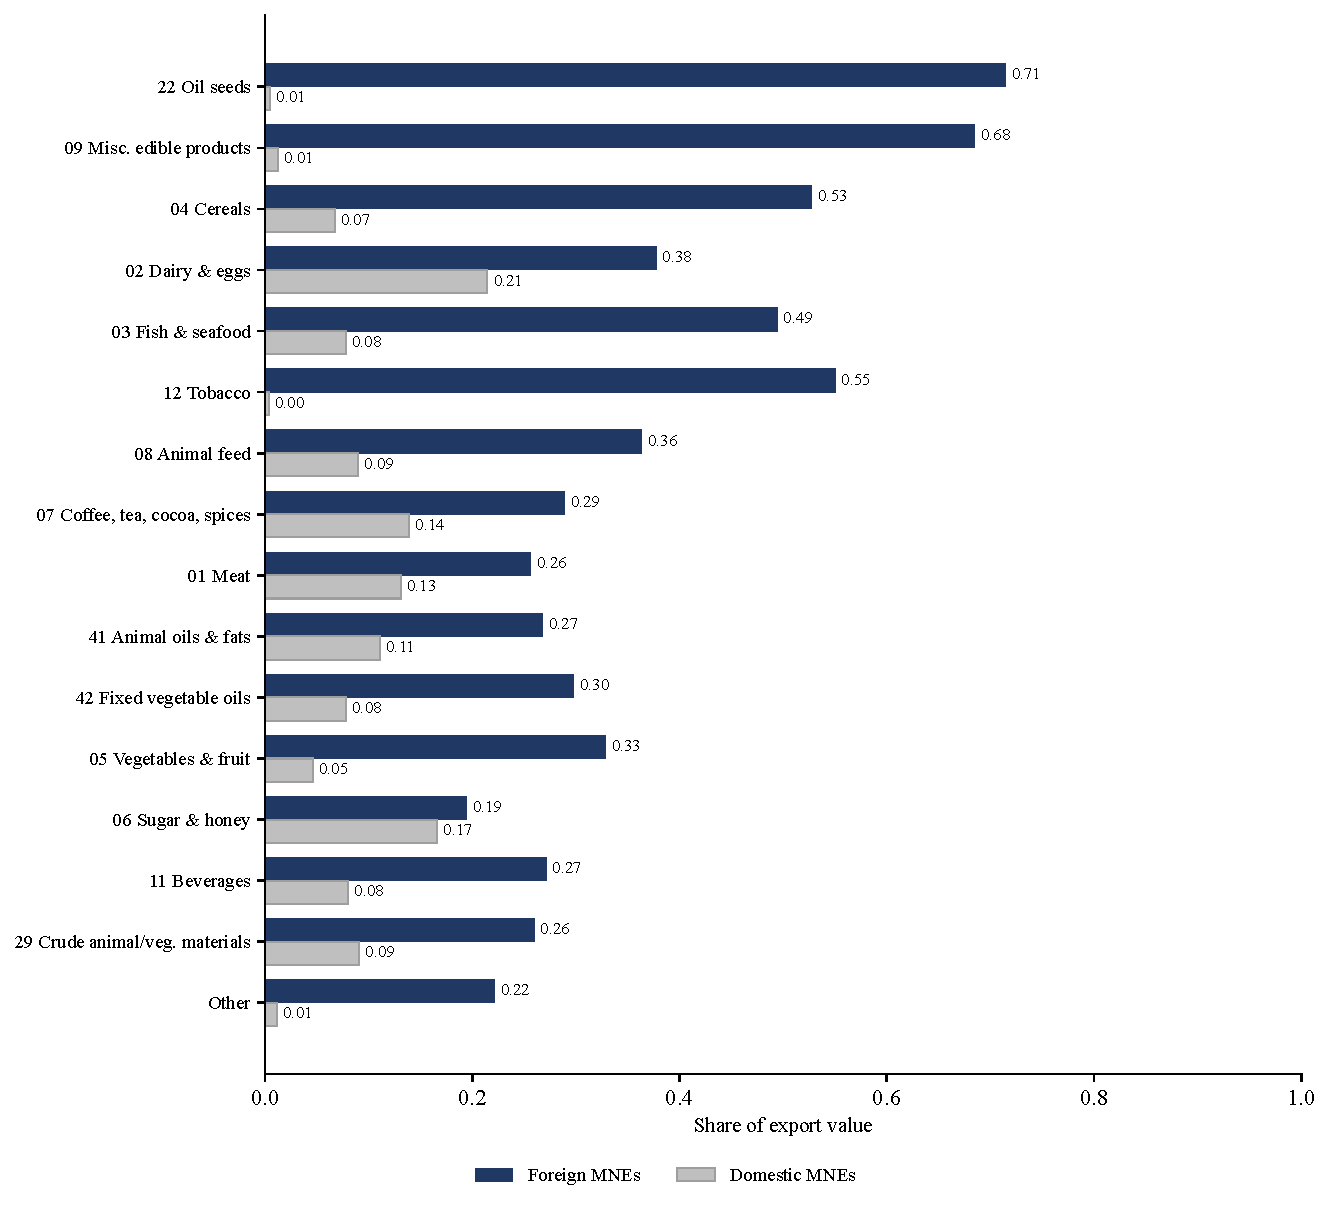
\includegraphics[width=0.85\linewidth,height=0.45\textheight,keepaspectratio]{figures/agro2018/fig_wp2_sitc2.pdf}

\begin{minipage}{0.9\linewidth}
\notesize
\vspace{0.6em}
\textit{Notes:} Shares of the agricultural export value of each SITC Rev.\,3 division in 2018, by type of exporter. Divisions are ordered by MNE share, from largest to smallest, with ``Other'' last.\\
\srcnote
\end{minipage}
\end{figure}

\FloatBarrier
\subsubsection*{Fact 2: Parents are based in a few countries}

The parents of foreign affiliates are based in a few countries (Figure~\ref{fig:parents}). In 2018, groups based in
the United States shipped 24 percent of the agricultural exports of foreign affiliates and Dutch groups 12 percent.
They were followed by groups whose parent is recorded in Switzerland (9 percent) and Liechtenstein (7 percent).
Spanish and Brazilian groups ship about 5 percent each and Saudi groups 4 percent. Tax havens and similar
jurisdictions, such as Switzerland, Liechtenstein, Luxembourg, Panama and Bermuda, together account for 26 percent.
Groups often hold their affiliates through companies located there, so the recorded parent country does not always
show where the activity of the group takes place.

Each parent country supplies a different set of markets. US groups supply 59 percent of the agricultural exports of
foreign affiliates that go to Argentina, most of them soybeans and soybean products shipped from Paraguay. They also
supply 35 percent of those that go to Vietnam and 22 percent of those that go to China, while Spanish groups supply
29 percent of those that go to Spain (Table~\ref{tab:pxd}). Few of these exports go back to the country of the
parent. Over 2012 to 2018, 4.5 percent of the agricultural exports of foreign affiliates went to the country of their
parent.

% ---- Figure: Agricultural exports of foreign multinationals, by parent country, 2018
\begin{figure}[htbp]
\centering
\caption{Agricultural exports of foreign multinationals, by parent country, 2018}
\label{fig:parents}
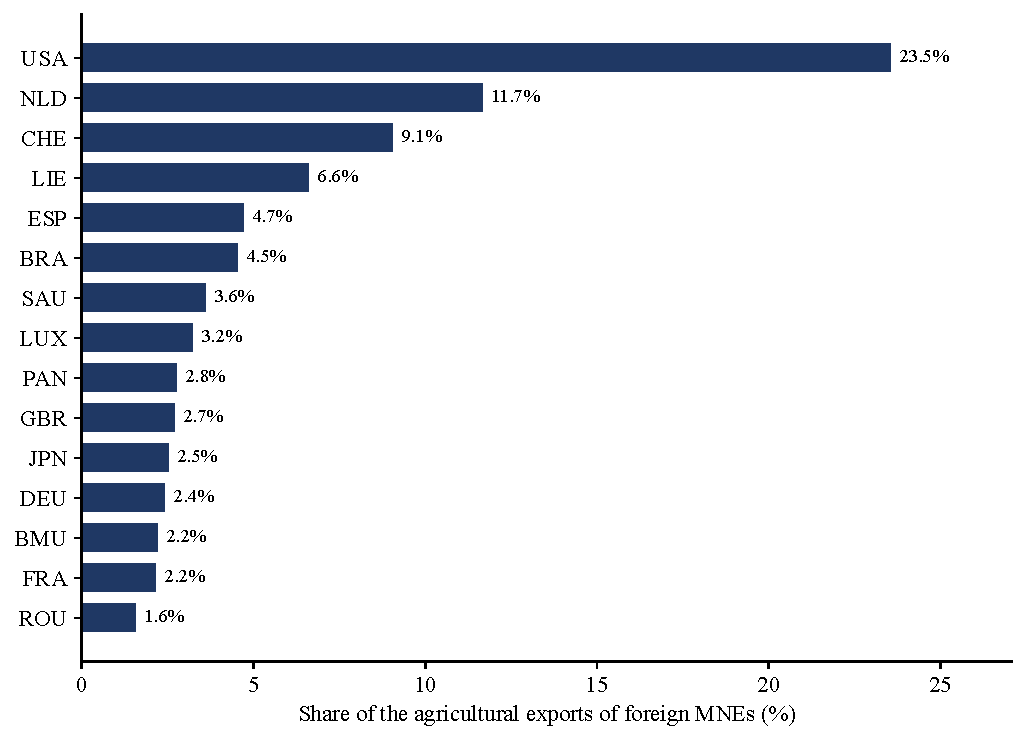
\includegraphics[width=0.78\linewidth,height=0.42\textheight,keepaspectratio]{figures/agro2018/fig_agp_parent_all.pdf}

\begin{minipage}{0.9\linewidth}
\notesize
\vspace{0.6em}
\textit{Notes:} Percent of the agricultural exports of foreign MNEs with a recorded parent country (88 percent of the total in 2018), by country of the parent. The fifteen largest parent countries, tax havens included.\\
\srcnote
\end{minipage}
\end{figure}

% ---- Table: Agricultural exports of foreign multinationals: top 10 destinations and top 10 parents, 2018
\begin{table}[htbp]
\centering
\caption{Agricultural exports of foreign multinationals: top 10 destinations and top 10 parents, 2018}
\label{tab:pxd}
{\footnotesize\setlength{\tabcolsep}{3pt}\setlength{\extrarowheight}{1pt}
\adjustbox{max width=\linewidth}{\begin{tabular}{lrrrrrrrrrrr}
\toprule
Top 10 parents / Top 10 destinations & USA & ARG & CHN & BRA & CHL & ESP & VNM & DZA & NLD & ITA & Other destinations \\
\midrule
USA & 17.4 & 59.2 & 22.0 & 7.2 & 26.3 & 5.2 & 34.7 & 26.7 & 13.2 & 4.2 & 21.2 \\
NLD & 1.7 & 10.2 & 11.9 & 10.3 & 17.1 & 4.7 & 19.4 & 25.6 & 9.4 & 27.0 & 12.9 \\
CHE & 1.5 & 0.1 & 0.7 & 16.1 & 14.8 & 4.9 & 11.5 & 26.8 & 0.9 & 17.4 & 13.0 \\
LIE & 1.0 & 0.0 & 4.6 & 11.0 & 10.3 & 4.6 & 18.4 & 7.9 & 0.9 & 4.8 & 9.1 \\
ESP & 7.6 & 0.1 & 6.3 & 1.1 & 1.5 & 29.3 & 2.3 & 0.2 & 13.3 & 7.8 & 3.3 \\
BRA & 4.8 & 2.1 & 12.9 & 4.9 & 1.1 & 2.1 & 3.2 & 4.2 & 6.5 & 4.0 & 3.3 \\
SAU & 1.7 & 0.0 & 5.9 & 2.3 & 15.5 & 1.6 & 4.6 & 0.0 & 3.0 & 3.5 & 4.1 \\
LUX & 1.2 & 0.0 & 1.6 & 16.0 & 1.3 & 9.5 & 0.7 & 0.1 & 0.2 & 6.4 & 2.9 \\
PAN & 6.0 & 0.1 & 4.7 & 0.4 & 0.6 & 3.5 & 0.5 & 0.0 & 5.1 & 0.5 & 3.0 \\
GBR & 1.6 & 0.1 & 5.6 & 3.9 & 1.8 & 2.5 & 0.8 & 0.1 & 2.9 & 0.7 & 3.3 \\
Other parents & 55.5 & 28.0 & 23.7 & 26.7 & 9.8 & 32.3 & 3.9 & 8.4 & 44.4 & 23.6 & 23.9 \\
\midrule
Total & 100.0 & 100.0 & 100.0 & 100.0 & 100.0 & 100.0 & 100.0 & 100.0 & 100.0 & 100.0 & 100.0 \\
\bottomrule
\end{tabular}
}}

\begin{minipage}{0.95\linewidth}
\notesize
\vspace{0.6em}
\textit{Notes:} Percent of the agricultural exports of foreign MNEs with a recorded parent country that go to each destination in 2018, by parent country. Each column adds to 100. The ten largest parent countries and the ten largest destinations account for 72 and 59 percent of these exports. The rest are grouped as other parents and other destinations.\\
\srcnote
\end{minipage}
\end{table}

\FloatBarrier
\subsubsection*{Fact 3: A few large groups ship most of the exports of foreign affiliates}

Most of the exports of foreign affiliates come from groups with very large networks (Figure~\ref{fig:network}). In
2018, 41 percent of parents had only one affiliate in the world. Yet the 15 percent of parents with more than 100
affiliates shipped 49 percent of the exports of foreign affiliates, and groups with more than ten affiliates shipped 79
percent.

% ---- Figure: Agricultural exports of foreign multinationals and number of parents, by size of the global network of the group, 2018
\begin{figure}[htbp]
\centering
\caption{Agricultural exports of foreign multinationals and number of parents, by size of the global network of the group, 2018}
\label{fig:network}
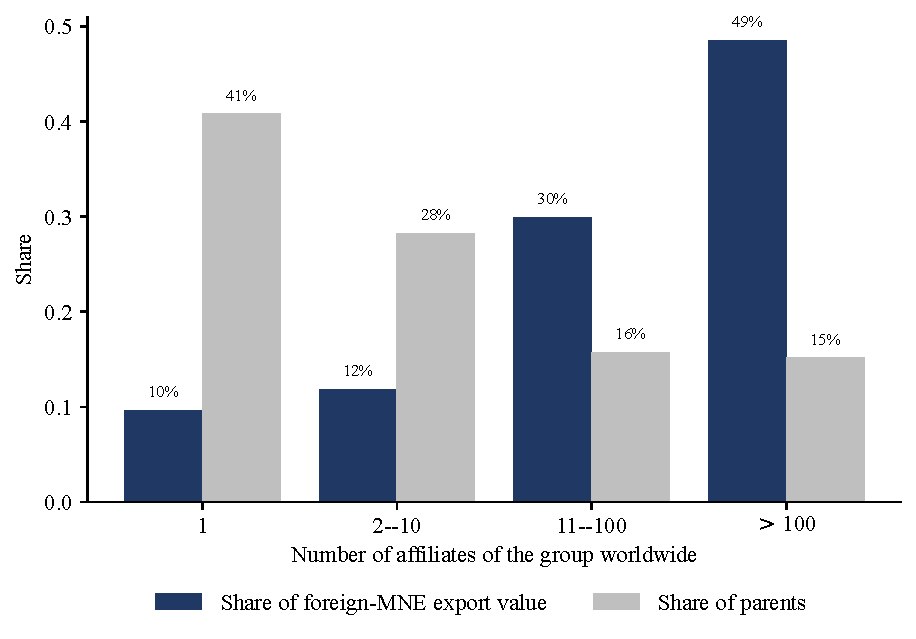
\includegraphics[width=0.78\linewidth,height=0.42\textheight,keepaspectratio]{figures/agro2018/fig_wp0_fig5_network.pdf}

\begin{minipage}{0.9\linewidth}
\notesize
\vspace{0.6em}
\textit{Notes:} Shares of the agricultural export value of foreign MNEs and of parents in 2018, by the number of affiliates the group has worldwide.\\
\srcnote
\end{minipage}
\end{figure}

\FloatBarrier
\subsubsection*{Fact 4: Exports are larger where more multinationals are present}

Exports are larger where more multinational firms export the same product to the same destination, and so are the
exports of local firms. To measure this association, we compare the exports of a product from an origin country to a
destination country in a year, an observation $odpy$, with the number of multinational firms that export it:
\begin{equation}\label{eq:presence}
\ln X_{odpy} = \beta \ln N_{odpy} + \delta + \varepsilon_{odpy},
\end{equation}
where $X_{odpy}$ is the value exported, $N_{odpy}$ is the number of multinational firms that export the product from
$o$ to $d$ in year $y$, and $\delta$ is a set of fixed effects. The coefficient $\beta$ is an elasticity. A 10 percent
higher number of multinationals is associated with exports about $10\beta$ percent larger. This is the intensive
margin, estimated on the observations with at least one multinational. At the extensive margin, $\ln N_{odpy}$ is
replaced by an indicator for at least one multinational, and its coefficient measures how much larger exports are, in
log points, where at least one multinational is present. The dependent variable is either the exports of all firms or
the exports of local firms only, which leave out the exports of the multinationals themselves.

Fixed effects absorb everything that is common to a group of observations, so each coefficient compares observations
within the same group. The tables add them from left to right. Column 1 has origin, destination, product and year
fixed effects. Column 2 replaces them with origin $\times$ year, destination $\times$ year and product fixed effects.
Column 3 has origin $\times$ destination $\times$ product fixed effects, so it compares the same product shipped from
the same origin to the same destination in different years, plus year fixed effects. Column 4 adds origin $\times$
destination $\times$ year fixed effects, which absorb changes over time in the trade between two countries. Column 5,
the strictest specification, adds origin $\times$ product $\times$ year and destination $\times$ product $\times$ year
fixed effects. These absorb, for example, the supply of each product in each origin and the demand for it in each
destination in each year. Standard errors are clustered by pair of origin and destination countries.

The regressions describe conditional correlations. Multinational firms choose the products and markets in which they
operate, and the same conditions that attract them may also attract other exporters. The estimates therefore do not
measure the effect of multinational presence on exports. The workbook that accompanies this note has one sheet for
each table, with every specification, its coefficients, standard errors, observations and $R^2$.

Most of the raw association reflects differences across combinations of origin, destination and product
(Table~\ref{tab:t1}). The elasticity of exports with respect to the number of multinationals is 2.20 with origin,
destination, product and year fixed effects, and 0.83 once the same origin, destination and product are followed over
time (Panel A, columns 1 and 3). It is 0.80 with origin $\times$ destination $\times$ year fixed effects and 0.54 in the
strictest specification. At the extensive margin, exports are 0.66 log points larger with at least one multinational
in column 3 and 0.56 log points larger in the strictest specification (Panel B). The association for local firms is
smaller, but it is positive and significant in every specification (Table~\ref{tab:t1local}). Their elasticity goes
from 1.58 in column 1 to 0.41, 0.37 and 0.16 in columns 3 to 5. The coefficient on the presence of at least one
multinational goes from 1.95 to 0.26, 0.24 and 0.10.

% ---- Table: Multinational presence and agricultural exports, all firms
\begin{table}[htbp]
\centering
\caption{Multinational presence and agricultural exports, all firms}
\label{tab:t1}
{\footnotesize\setlength{\tabcolsep}{4pt}\setlength{\extrarowheight}{1pt}
\adjustbox{max width=\linewidth}{\begin{tabular}{l*{5}{c}}
\toprule
 & (1) & (2) & (3) & (4) & (5) \\
\midrule
\multicolumn{6}{l}{\textit{Panel A. Intensive margin: observations with at least one MNE}} \\
$\ln$(number of MNEs) & 2.200*** & 2.205*** & 0.830*** & 0.797*** & 0.536*** \\
 & (0.029) & (0.029) & (0.023) & (0.022) & (0.034) \\
Observations (Panel A) & 101,098 & 100,983 & 89,828 & 88,037 & 30,271 \\
$R^2$ & 0.503 & 0.512 & 0.907 & 0.917 & 0.970 \\
\midrule
\multicolumn{6}{l}{\textit{Panel B. Extensive margin: all observations}} \\
At least one MNE & 1.818*** & 1.820*** & 0.658*** & 0.655*** & 0.565*** \\
 & (0.065) & (0.065) & (0.027) & (0.026) & (0.038) \\
Observations (Panel B) & 198,231 & 198,142 & 177,525 & 175,847 & 85,000 \\
$R^2$ & 0.397 & 0.405 & 0.871 & 0.879 & 0.947 \\
\midrule
Origin FE & $\checkmark$ &  &  &  &  \\
Destination FE & $\checkmark$ &  &  &  &  \\
Product FE & $\checkmark$ & $\checkmark$ &  &  &  \\
Year FE & $\checkmark$ &  & $\checkmark$ &  &  \\
Origin $\times$ year FE &  & $\checkmark$ &  &  &  \\
Destination $\times$ year FE &  & $\checkmark$ &  &  &  \\
Origin $\times$ destination $\times$ product FE &  &  & $\checkmark$ & $\checkmark$ & $\checkmark$ \\
Origin $\times$ destination $\times$ year FE &  &  &  & $\checkmark$ & $\checkmark$ \\
Origin $\times$ product $\times$ year FE &  &  &  &  & $\checkmark$ \\
Destination $\times$ product $\times$ year FE &  &  &  &  & $\checkmark$ \\
\bottomrule
\end{tabular}
}}

\begin{minipage}{0.95\linewidth}
\notesize
\vspace{0.6em}
\textit{Notes:} Regression at the level of origin country, destination country, product and year (equation~\ref{eq:presence}). Agricultural products, 2012 to 2018. Dependent variable: $\ln$ exports of all firms. Panel A: $\ln$ number of MNEs, observations with at least one MNE. Panel B: indicator for at least one MNE, all observations. Standard errors clustered by pair of origin and destination countries in parentheses. *** $p<0.01$, ** $p<0.05$, * $p<0.1$.\\
\srcnote
\end{minipage}
\end{table}

% ---- Table: Multinational presence and agricultural exports, local firms
\begin{table}[htbp]
\centering
\caption{Multinational presence and agricultural exports, local firms}
\label{tab:t1local}
{\footnotesize\setlength{\tabcolsep}{4pt}\setlength{\extrarowheight}{1pt}
\adjustbox{max width=\linewidth}{\begin{tabular}{l*{5}{c}}
\toprule
 & (1) & (2) & (3) & (4) & (5) \\
\midrule
\multicolumn{6}{l}{\textit{Panel A. Intensive margin: observations with at least one MNE}} \\
$\ln$(number of MNEs) & 1.578*** & 1.589*** & 0.411*** & 0.375*** & 0.156*** \\
 & (0.035) & (0.035) & (0.029) & (0.028) & (0.049) \\
Observations (Panel A) & 59,848 & 59,708 & 54,234 & 52,515 & 16,372 \\
$R^2$ & 0.496 & 0.506 & 0.879 & 0.892 & 0.969 \\
\midrule
\multicolumn{6}{l}{\textit{Panel B. Extensive margin: all observations}} \\
At least one MNE & 1.947*** & 1.948*** & 0.262*** & 0.239*** & 0.102*** \\
 & (0.064) & (0.063) & (0.023) & (0.021) & (0.034) \\
Observations (Panel B) & 156,990 & 156,915 & 138,938 & 137,240 & 58,746 \\
$R^2$ & 0.424 & 0.434 & 0.867 & 0.876 & 0.948 \\
\midrule
Origin FE & $\checkmark$ &  &  &  &  \\
Destination FE & $\checkmark$ &  &  &  &  \\
Product FE & $\checkmark$ & $\checkmark$ &  &  &  \\
Year FE & $\checkmark$ &  & $\checkmark$ &  &  \\
Origin $\times$ year FE &  & $\checkmark$ &  &  &  \\
Destination $\times$ year FE &  & $\checkmark$ &  &  &  \\
Origin $\times$ destination $\times$ product FE &  &  & $\checkmark$ & $\checkmark$ & $\checkmark$ \\
Origin $\times$ destination $\times$ year FE &  &  &  & $\checkmark$ & $\checkmark$ \\
Origin $\times$ product $\times$ year FE &  &  &  &  & $\checkmark$ \\
Destination $\times$ product $\times$ year FE &  &  &  &  & $\checkmark$ \\
\bottomrule
\end{tabular}
}}

\begin{minipage}{0.95\linewidth}
\notesize
\vspace{0.6em}
\textit{Notes:} Regressions as in Table~\ref{tab:t1}. Dependent variable: $\ln$ exports of local firms, which leave out the exports of the multinationals themselves. Standard errors clustered by pair of origin and destination countries in parentheses. *** $p<0.01$, ** $p<0.05$, * $p<0.1$.\\
\srcnote
\end{minipage}
\end{table}

The larger exports of local firms come mainly from more local exporters rather than from larger sales per exporter
(Table~\ref{tab:mneprod}). This table restricts the sample to the products in which multinationals operate, that is,
those that at least one multinational from the same origin exports in some year between 2012 and 2018. They account
for 97 percent of the observations and 99.5 percent of the value. At the intensive margin the sample does not change,
since every observation with a multinational belongs to one of these products, and at the extensive margin the
estimates for total exports and for the exports of local firms are practically the same as before (columns 1 to 4). We then split the exports of local firms
into the number of local exporters and the exports per local exporter. A 10 percent higher number of multinationals
is associated with 2.3 percent more local exporters and 1.5 percent higher exports per local exporter (columns 5 and
7). In the strictest specification, the first remains significant (1.1 percent) and the second does not (0.5
percent). The extensive margin shows the same pattern (Panel B).

% ---- Table: Multinational presence and the exports of local firms: number of exporters and exports per exporter
\begin{table}[htbp]
\centering
\caption{Multinational presence and the exports of local firms: number of exporters and exports per exporter}
\label{tab:mneprod}
{\footnotesize\setlength{\tabcolsep}{3pt}\setlength{\extrarowheight}{1pt}
\adjustbox{max width=\linewidth}{\begin{tabular}{l*{8}{c}}
\toprule
 & \multicolumn{2}{c}{$\ln$ exports,} & \multicolumn{2}{c}{$\ln$ exports,} & \multicolumn{2}{c}{$\ln$ number of} & \multicolumn{2}{c}{$\ln$ exports per} \\
 & \multicolumn{2}{c}{all firms} & \multicolumn{2}{c}{local firms} & \multicolumn{2}{c}{local exporters} & \multicolumn{2}{c}{local exporter} \\
\cmidrule(lr){2-3}\cmidrule(lr){4-5}\cmidrule(lr){6-7}\cmidrule(lr){8-9}
 & (1) & (2) & (3) & (4) & (5) & (6) & (7) & (8) \\
\midrule
\multicolumn{9}{l}{\textit{Panel A. Intensive margin: observations with at least one MNE}} \\
$\ln$(number of MNEs) & 0.796*** & 0.553*** & 0.373*** & 0.178*** & 0.227*** & 0.119*** & 0.146*** & 0.060 \\
 & (0.022) & (0.031) & (0.028) & (0.049) & (0.012) & (0.017) & (0.020) & (0.042) \\
Observations (Panel A) & 88,843 & 33,008 & 53,011 & 18,118 & 53,011 & 18,118 & 53,011 & 18,118 \\
$R^2$ & 0.916 & 0.969 & 0.892 & 0.967 & 0.894 & 0.975 & 0.877 & 0.957 \\
\midrule
\multicolumn{9}{l}{\textit{Panel B. Extensive margin: all observations}} \\
At least one MNE & 0.658*** & 0.571*** & 0.242*** & 0.088*** & 0.127*** & 0.058*** & 0.115*** & 0.030 \\
 & (0.026) & (0.036) & (0.021) & (0.030) & (0.007) & (0.009) & (0.018) & (0.030) \\
Observations (Panel B) & 172,780 & 89,211 & 133,856 & 61,746 & 133,856 & 61,746 & 133,856 & 61,746 \\
$R^2$ & 0.878 & 0.946 & 0.875 & 0.947 & 0.861 & 0.954 & 0.864 & 0.937 \\
\midrule
Origin $\times$ destination $\times$ product FE & $\checkmark$ & $\checkmark$ & $\checkmark$ & $\checkmark$ & $\checkmark$ & $\checkmark$ & $\checkmark$ & $\checkmark$ \\
Origin $\times$ destination $\times$ year FE & $\checkmark$ & $\checkmark$ & $\checkmark$ & $\checkmark$ & $\checkmark$ & $\checkmark$ & $\checkmark$ & $\checkmark$ \\
Origin $\times$ product $\times$ year FE &  & $\checkmark$ &  & $\checkmark$ &  & $\checkmark$ &  & $\checkmark$ \\
Destination $\times$ product $\times$ year FE &  & $\checkmark$ &  & $\checkmark$ &  & $\checkmark$ &  & $\checkmark$ \\
\bottomrule
\end{tabular}
}}

\begin{minipage}{0.95\linewidth}
\notesize
\vspace{0.6em}
\textit{Notes:} Regression at the level of origin country, destination country, product and year. Agricultural products, 2012 to 2018, restricted to the products that at least one MNE from the same origin exports in some year. Odd columns have the fixed effects of column 4 of Table~\ref{tab:t1} and even columns those of column 5, the strictest specification. The workbook reports the five specifications of Table~\ref{tab:t1} for each dependent variable. Panel A: $\ln$ number of MNEs, observations with at least one MNE. Panel B: indicator for at least one MNE, all observations. Standard errors clustered by pair of origin and destination countries in parentheses. *** $p<0.01$, ** $p<0.05$, * $p<0.1$.\\
\srcnote
\end{minipage}
\end{table}

\FloatBarrier
\subsubsection*{Fact 5: The association is stronger for field crops and for capital intensive farm products}

Multinationals ship a larger share of the exports of large and mechanized agriculture. Over 2012 to 2018, they account
for 51.0 percent of the exports of field crops and 40.8 percent of those of horticultural and plantation crops. They
also account for 59.5 percent of the exports of farm products with high capital intensity, against 38.4 percent of the
other farm products. Among processed products, capital intensity makes little difference. The share is 47.1 percent
with high and 48.0 percent with low capital intensity (Table~\ref{tab:groups}).

% ---- Table: Agricultural exports and multinational shares, by type of production and capital intensity
\begin{table}[htbp]
\centering
\caption{Agricultural exports and multinational shares, by type of production and capital intensity}
\label{tab:groups}
{\footnotesize\setlength{\tabcolsep}{4pt}\setlength{\extrarowheight}{1pt}
\adjustbox{max width=\linewidth}{\begin{tabular}{lrrrrr}
\toprule
Group & Products & Share of exports (\%) & MNE share (\%) & Foreign MNE share (\%) & Capital per worker (US\$ thousand) \\
\midrule
\textit{Type of production} &  &  &  &  &  \\
Horticultural and plantation crops & 306 & 27.6 & 40.8 & 33.5 &  \\
Field crops & 202 & 47.5 & 51.0 & 42.2 &  \\
Livestock and fisheries & 395 & 19.2 & 46.9 & 34.3 &  \\
Other processed food and beverages & 78 & 5.7 & 61.1 & 51.4 &  \\
\textit{Capital intensity} &  &  &  &  &  \\
Farm stage, high & 91 & 20.1 & 59.5 & 54.4 & 344 \\
Farm stage, low & 198 & 20.3 & 38.4 & 30.9 & 25 \\
Processing stage, high & 284 & 41.5 & 47.1 & 36.1 & 290 \\
Processing stage, low & 215 & 9.7 & 48.0 & 37.4 & 72 \\
Not classified & 193 & 8.5 & 47.9 & 36.0 &  \\
\bottomrule
\end{tabular}
}}

\begin{minipage}{0.95\linewidth}
\notesize
\vspace{0.6em}
\textit{Notes:} Agricultural exports of the nine countries, 2012 to 2018. Types of production follow the crop groups of the FAO Indicative Crop Classification. Capital intensity at the farm stage is machinery and equipment per hired worker of the US type of farm (2017 Census of Agriculture). At the processing stage, it is equipment capital per employee of the US industry (NBER and CES database, average of 2012 to 2018). It is high when it is above the ratio of the stage as a whole. Capital per worker is the average of the group weighted by exports, in US\$ thousand. Not classified: products of other industries, mainly fish, seafood and fish meal.\\
\textit{Source:} Authors' calculations based on customs data matched to Orbis (Bureau van Dijk) and Dun \& Bradstreet, FAO, USDA NASS, and NBER and CES.
\end{minipage}
\end{table}

The association between multinational presence and exports is also stronger in these products
(Tables~\ref{tab:crop} and~\ref{tab:capital}). To compare groups, we replace $\ln N_{odpy}$ in
equation~(\ref{eq:presence}) with its products with an indicator for each group, so each coefficient is the
elasticity of one group. The group itself does not enter on its own, since the origin $\times$ destination $\times$
product fixed effects absorb it. With origin $\times$ destination $\times$ year fixed effects, the elasticity is 0.98
for field crops and 0.67 for horticultural and plantation crops. In the strictest specification it is 0.96 against
0.47. Both differences are significant at the 1 percent level (Table~\ref{tab:crop}, Panel A, columns 4 and 5). For
local firms, the elasticity is 0.52 in field crops and 0.32 in horticultural and plantation crops in column 4. This
difference is significant at the 1 percent level, but not in the strictest specification (Panel B).

% ---- Table: Multinational presence and agricultural exports, by type of production
\begin{table}[htbp]
\centering
\caption{Multinational presence and agricultural exports, by type of production}
\label{tab:crop}
{\footnotesize\setlength{\tabcolsep}{4pt}\setlength{\extrarowheight}{1pt}
\adjustbox{max width=\linewidth}{\begin{tabular}{l*{5}{c}}
\toprule
 & (1) & (2) & (3) & (4) & (5) \\
\midrule
\multicolumn{6}{l}{\textit{Panel A. Dependent variable: $\ln$ exports, all firms}} \\
$\ln$(number of MNEs) $\times$ horticultural and plantation crops & 2.106*** & 2.113*** & 0.711*** & 0.677*** & 0.485*** \\
 & (0.044) & (0.044) & (0.029) & (0.026) & (0.040) \\
$\ln$(number of MNEs) $\times$ field crops & 2.462*** & 2.459*** & 1.035*** & 1.008*** & 0.989*** \\
 & (0.057) & (0.057) & (0.043) & (0.044) & (0.103) \\
$\ln$(number of MNEs) $\times$ livestock and fisheries & 2.123*** & 2.125*** & 0.958*** & 0.915*** & 0.626*** \\
 & (0.044) & (0.044) & (0.036) & (0.038) & (0.065) \\
$\ln$(number of MNEs) $\times$ other processed food & 2.349*** & 2.360*** & 0.739*** & 0.708*** & 0.483*** \\
 & (0.071) & (0.071) & (0.044) & (0.043) & (0.071) \\
$p$ value: field crops = horticultural and plantation crops & 0.000 & 0.000 & 0.000 & 0.000 & 0.000 \\
Observations (Panel A) & 101,847 & 101,732 & 90,632 & 88,843 & 33,008 \\
$R^2$ & 0.500 & 0.509 & 0.907 & 0.917 & 0.969 \\
\midrule
\multicolumn{6}{l}{\textit{Panel B. Dependent variable: $\ln$ exports, local firms}} \\
$\ln$(number of MNEs) $\times$ horticultural and plantation crops & 1.625*** & 1.638*** & 0.352*** & 0.311*** & 0.174*** \\
 & (0.046) & (0.046) & (0.040) & (0.037) & (0.064) \\
$\ln$(number of MNEs) $\times$ field crops & 1.779*** & 1.793*** & 0.577*** & 0.550*** & 0.321 \\
 & (0.049) & (0.049) & (0.047) & (0.049) & (0.195) \\
$\ln$(number of MNEs) $\times$ livestock and fisheries & 1.403*** & 1.406*** & 0.541*** & 0.507*** & 0.251** \\
 & (0.050) & (0.051) & (0.046) & (0.050) & (0.127) \\
$\ln$(number of MNEs) $\times$ other processed food & 1.346*** & 1.361*** & 0.207*** & 0.146** & 0.099 \\
 & (0.083) & (0.084) & (0.067) & (0.066) & (0.100) \\
$p$ value: field crops = horticultural and plantation crops & 0.014 & 0.014 & 0.000 & 0.000 & 0.469 \\
Observations (Panel B) & 60,343 & 60,204 & 54,751 & 53,011 & 18,118 \\
$R^2$ & 0.495 & 0.505 & 0.879 & 0.892 & 0.967 \\
\midrule
Origin FE & $\checkmark$ &  &  &  &  \\
Destination FE & $\checkmark$ &  &  &  &  \\
Product FE & $\checkmark$ & $\checkmark$ &  &  &  \\
Year FE & $\checkmark$ &  & $\checkmark$ &  &  \\
Origin $\times$ year FE &  & $\checkmark$ &  &  &  \\
Destination $\times$ year FE &  & $\checkmark$ &  &  &  \\
Origin $\times$ destination $\times$ product FE &  &  & $\checkmark$ & $\checkmark$ & $\checkmark$ \\
Origin $\times$ destination $\times$ year FE &  &  &  & $\checkmark$ & $\checkmark$ \\
Origin $\times$ product $\times$ year FE &  &  &  &  & $\checkmark$ \\
Destination $\times$ product $\times$ year FE &  &  &  &  & $\checkmark$ \\
\bottomrule
\end{tabular}
}}

\begin{minipage}{0.95\linewidth}
\notesize
\vspace{0.6em}
\textit{Notes:} Regressions as in Table~\ref{tab:t1}, Panel A, with $\ln$ number of MNEs interacted with an indicator for each type of production and no term without interaction. Observations with at least one MNE. The $p$ value tests that the coefficients of field crops and of horticultural and plantation crops are equal. Table~\ref{tab:crop_ext} in the Appendix reports the extensive margin. Standard errors clustered by pair of origin and destination countries in parentheses. *** $p<0.01$, ** $p<0.05$, * $p<0.1$.\\
\textit{Source:} Authors' calculations based on customs data matched to Orbis (Bureau van Dijk) and Dun \& Bradstreet. Crop groups from the FAO Indicative Crop Classification.
\end{minipage}
\end{table}

Capital intensity gives a similar result at the farm stage. With origin $\times$ destination $\times$ year fixed
effects, the elasticity is 1.05 for farm products with high capital intensity and 0.76 for the other farm products. In
the strictest specification it is 0.82 against 0.57. Both differences are significant (Table~\ref{tab:capital},
Panel A, columns 4 and 5). Among processed products, the elasticities of the two groups are nearly equal, 0.75 and
0.76. For local firms, the elasticity is 0.66 in farm products with high capital intensity and 0.43 in the other farm
products in column 4. In the strictest specification, the first is no longer significant and the difference is not
significant either (Panel B).

The extensive margin gives a similar picture (Tables~\ref{tab:crop_ext} and~\ref{tab:capital_ext} in the Appendix).
Once origin $\times$ destination $\times$ product fixed effects are included, the presence of at least one
multinational shows a stronger association with exports in field crops than in horticultural and plantation crops.
The difference is significant with origin $\times$ destination $\times$ year fixed effects but not in the strictest
specification. In these two specifications, the differences by capital intensity are significant only for local
firms at the farm stage, with origin $\times$ destination $\times$ year fixed effects. Field crops and farm products
with high capital intensity are produced at a large scale and are shipped in bulk through storage, crushing and port
facilities that large traders operate. This is consistent with a closer link between the presence of multinationals
and exports in these products.

% ---- Table: Multinational presence and agricultural exports, by capital intensity
\begin{table}[htbp]
\centering
\caption{Multinational presence and agricultural exports, by capital intensity}
\label{tab:capital}
{\footnotesize\setlength{\tabcolsep}{4pt}\setlength{\extrarowheight}{1pt}
\adjustbox{max width=\linewidth}{\begin{tabular}{l*{5}{c}}
\toprule
 & (1) & (2) & (3) & (4) & (5) \\
\midrule
\multicolumn{6}{l}{\textit{Panel A. Dependent variable: $\ln$ exports, all firms}} \\
$\ln$(number of MNEs) $\times$ farm stage, high capital intensity & 2.366*** & 2.362*** & 1.132*** & 1.110*** & 1.093*** \\
 & (0.067) & (0.067) & (0.058) & (0.060) & (0.129) \\
$\ln$(number of MNEs) $\times$ farm stage, low capital intensity & 2.117*** & 2.121*** & 0.712*** & 0.664*** & 0.498*** \\
 & (0.052) & (0.052) & (0.036) & (0.033) & (0.052) \\
$\ln$(number of MNEs) $\times$ processing stage, high capital intensity & 2.271*** & 2.280*** & 0.787*** & 0.760*** & 0.517*** \\
 & (0.037) & (0.037) & (0.029) & (0.028) & (0.051) \\
$\ln$(number of MNEs) $\times$ processing stage, low capital intensity & 2.103*** & 2.107*** & 0.922*** & 0.880*** & 0.571*** \\
 & (0.047) & (0.047) & (0.039) & (0.040) & (0.058) \\
$\ln$(number of MNEs) $\times$ not classified & 2.070*** & 2.071*** & 0.861*** & 0.872*** & -0.020 \\
 & (0.186) & (0.187) & (0.140) & (0.144) & (0.509) \\
$p$ value: farm stage, high = low & 0.004 & 0.005 & 0.000 & 0.000 & 0.000 \\
$p$ value: processing stage, high = low & 0.002 & 0.002 & 0.003 & 0.012 & 0.446 \\
Observations (Panel A) & 101,847 & 101,732 & 90,632 & 88,843 & 33,008 \\
$R^2$ & 0.500 & 0.509 & 0.907 & 0.917 & 0.969 \\
\midrule
\multicolumn{6}{l}{\textit{Panel B. Dependent variable: $\ln$ exports, local firms}} \\
$\ln$(number of MNEs) $\times$ farm stage, high capital intensity & 1.836*** & 1.853*** & 0.708*** & 0.692*** & 0.491** \\
 & (0.062) & (0.062) & (0.067) & (0.070) & (0.225) \\
$\ln$(number of MNEs) $\times$ farm stage, low capital intensity & 1.692*** & 1.701*** & 0.398*** & 0.344*** & 0.252*** \\
 & (0.056) & (0.055) & (0.045) & (0.041) & (0.074) \\
$\ln$(number of MNEs) $\times$ processing stage, high capital intensity & 1.502*** & 1.515*** & 0.281*** & 0.235*** & 0.031 \\
 & (0.046) & (0.046) & (0.038) & (0.037) & (0.087) \\
$\ln$(number of MNEs) $\times$ processing stage, low capital intensity & 1.374*** & 1.381*** & 0.515*** & 0.493*** & 0.275*** \\
 & (0.056) & (0.057) & (0.047) & (0.051) & (0.094) \\
$\ln$(number of MNEs) $\times$ not classified & 1.222*** & 1.232*** & 0.541*** & 0.546*** & 0.304 \\
 & (0.245) & (0.244) & (0.142) & (0.154) & (0.500) \\
$p$ value: farm stage, high = low & 0.073 & 0.058 & 0.000 & 0.000 & 0.328 \\
$p$ value: processing stage, high = low & 0.039 & 0.033 & 0.000 & 0.000 & 0.059 \\
Observations (Panel B) & 60,343 & 60,204 & 54,751 & 53,011 & 18,118 \\
$R^2$ & 0.495 & 0.505 & 0.879 & 0.892 & 0.967 \\
\midrule
Origin FE & $\checkmark$ &  &  &  &  \\
Destination FE & $\checkmark$ &  &  &  &  \\
Product FE & $\checkmark$ & $\checkmark$ &  &  &  \\
Year FE & $\checkmark$ &  & $\checkmark$ &  &  \\
Origin $\times$ year FE &  & $\checkmark$ &  &  &  \\
Destination $\times$ year FE &  & $\checkmark$ &  &  &  \\
Origin $\times$ destination $\times$ product FE &  &  & $\checkmark$ & $\checkmark$ & $\checkmark$ \\
Origin $\times$ destination $\times$ year FE &  &  &  & $\checkmark$ & $\checkmark$ \\
Origin $\times$ product $\times$ year FE &  &  &  &  & $\checkmark$ \\
Destination $\times$ product $\times$ year FE &  &  &  &  & $\checkmark$ \\
\bottomrule
\end{tabular}
}}

\begin{minipage}{0.95\linewidth}
\notesize
\vspace{0.6em}
\textit{Notes:} Regressions as in Table~\ref{tab:t1}, Panel A, with $\ln$ number of MNEs interacted with an indicator for each group of capital intensity (Table~\ref{tab:groups}) and no term without interaction. Observations with at least one MNE. The $p$ values test that the coefficients of high and low capital intensity are equal within each stage. Table~\ref{tab:capital_ext} in the Appendix reports the extensive margin. Standard errors clustered by pair of origin and destination countries in parentheses. *** $p<0.01$, ** $p<0.05$, * $p<0.1$.\\
\textit{Source:} Authors' calculations based on customs data matched to Orbis (Bureau van Dijk) and Dun \& Bradstreet, USDA NASS, and NBER and CES.
\end{minipage}
\end{table}

\FloatBarrier
\subsubsection*{Fact 6: The exports of multinationals do not fall less with distance}

The exports of multinationals do not fall less with distance than those of local firms once the same firm is
compared across destinations. This fact comes from a regression at the level of the firm, destination, product and
year:
\begin{equation}\label{eq:dist}
\ln x_{fodpy} = \alpha \ln D_{od} + \gamma \left(M_{f} \times \ln D_{od}\right) + \theta M_f + \delta + u_{fodpy},
\end{equation}
where $x_{fodpy}$ is the value of product $p$ exported by firm $f$ from country $o$ to country $d$ in year $y$, $D_{od}$
is the distance between the two countries from the CEPII gravity database, and $M_f$ equals one if the firm is a
multinational affiliate. The coefficient $\alpha$ measures how the exports of local firms vary with distance, and
$\gamma$ how this differs for multinationals. A positive $\gamma$ means that the exports of multinationals fall less
with distance. Columns 1 and 2 of Table~\ref{tab:dist} have origin, destination, product and year fixed effects, and
column 3 has origin $\times$ year, destination $\times$ year and product fixed effects. Columns 4 to 7 add firm, firm
$\times$ product, firm $\times$ year and firm $\times$ product $\times$ year fixed effects. Column 8 replaces the
destination $\times$ year fixed effects with destination $\times$ product $\times$ year fixed effects. A firm fixed
effect absorbs $M_f$, and $\gamma$ then compares the exports of the same firm to destinations at different distances.

In a specification that leaves out the MNE indicator $M_f$, as in the previous version of this note, the interaction
is positive, 0.034, and suggests that the exports of multinationals fall less with distance (Table~\ref{tab:dist},
column 1). This result is not robust. Multinationals export more than local firms at every distance, and since $\ln
D_{od}$ is always large and positive, the interaction picks up this difference in levels. Once $M_f$ is included,
multinationals export 0.82 log points more than local firms and the interaction becomes negative. The distance
elasticity of the exports of multinationals is then larger in absolute value than that of local firms, by 0.061
(column 2). With firm fixed effects, the interaction is small and not significant (columns 4 to 8). The exception is
the specification with firm $\times$ product fixed effects (column 5), where the difference is 0.035 and significant at
the 10 percent level. Splitting multinationals by whether the group is present at the destination, through an
affiliate there or because it is the country of the parent, gives the same pattern (Panel B). The coefficient on
distance grows in absolute value from 0.21 to 0.63 as fixed effects are added.

% ---- Table: Distance and firm agricultural exports, all firms
\begin{table}[htbp]
\centering
\caption{Distance and firm agricultural exports, all firms}
\label{tab:dist}
{\footnotesize\setlength{\tabcolsep}{3pt}\setlength{\extrarowheight}{1pt}
\adjustbox{max width=\linewidth}{\begin{tabular}{l*{8}{c}}
\toprule
 & (1) & (2) & (3) & (4) & (5) & (6) & (7) & (8) \\
\midrule
\multicolumn{9}{l}{\textit{Panel A. All multinationals}} \\
$\ln$ distance & -0.212*** & -0.185** & -0.196** & -0.400*** & -0.553*** & -0.422*** & -0.594*** & -0.629*** \\
 & (0.081) & (0.081) & (0.078) & (0.047) & (0.055) & (0.049) & (0.056) & (0.043) \\
$\ln$ distance $\times$ MNE & 0.034*** & -0.061** & -0.059** & -0.017 & -0.035* & -0.010 & -0.023 & -0.011 \\
 & (0.003) & (0.028) & (0.028) & (0.019) & (0.019) & (0.020) & (0.020) & (0.019) \\
MNE &  & 0.821*** & 0.799*** &  &  &  &  &  \\
 &  & (0.257) & (0.253) &  &  &  &  &  \\
Observations (Panel A) & 693,518 & 693,518 & 693,447 & 683,847 & 637,743 & 662,745 & 516,770 & 461,042 \\
$R^2$ & 0.372 & 0.372 & 0.377 & 0.597 & 0.687 & 0.626 & 0.669 & 0.764 \\
\midrule
\multicolumn{9}{l}{\textit{Panel B. Multinationals by presence at the destination}} \\
$\ln$ distance & -0.207*** & -0.180** & -0.191** & -0.399*** & -0.550*** & -0.420*** & -0.592*** & -0.627*** \\
 & (0.080) & (0.081) & (0.077) & (0.047) & (0.055) & (0.049) & (0.056) & (0.043) \\
$\ln$ distance $\times$ MNE, present & 0.087*** & -0.130** & -0.125** & 0.002 & -0.002 & 0.010 & 0.013 & 0.020 \\
 & (0.008) & (0.054) & (0.053) & (0.022) & (0.020) & (0.023) & (0.021) & (0.020) \\
$\ln$ distance $\times$ MNE, not present & 0.025*** & -0.025 & -0.023 & -0.019 & -0.039** & -0.013 & -0.027 & -0.014 \\
 & (0.004) & (0.033) & (0.032) & (0.019) & (0.019) & (0.020) & (0.020) & (0.019) \\
MNE, present at destination &  & 1.846*** & 1.799*** &  &  &  &  &  \\
 &  & (0.479) & (0.473) &  &  &  &  &  \\
MNE, not present at destination &  & 0.430 & 0.413 &  &  &  &  &  \\
 &  & (0.296) & (0.293) &  &  &  &  &  \\
Observations (Panel B) & 693,518 & 693,518 & 693,447 & 683,847 & 637,743 & 662,745 & 516,770 & 461,042 \\
$R^2$ & 0.373 & 0.373 & 0.378 & 0.597 & 0.687 & 0.626 & 0.669 & 0.764 \\
\midrule
Origin FE & $\checkmark$ & $\checkmark$ &  &  &  &  &  &  \\
Destination FE & $\checkmark$ & $\checkmark$ &  &  &  &  &  &  \\
Product FE & $\checkmark$ & $\checkmark$ & $\checkmark$ & $\checkmark$ &  & $\checkmark$ &  &  \\
Year FE & $\checkmark$ & $\checkmark$ &  &  &  &  &  &  \\
Origin $\times$ year FE &  &  & $\checkmark$ & $\checkmark$ & $\checkmark$ &  &  &  \\
Destination $\times$ year FE &  &  & $\checkmark$ & $\checkmark$ & $\checkmark$ & $\checkmark$ & $\checkmark$ &  \\
Firm FE &  &  &  & $\checkmark$ &  &  &  &  \\
Firm $\times$ product FE &  &  &  &  & $\checkmark$ &  &  &  \\
Firm $\times$ year FE &  &  &  &  &  & $\checkmark$ &  &  \\
Firm $\times$ product $\times$ year FE &  &  &  &  &  &  & $\checkmark$ & $\checkmark$ \\
Destination $\times$ product $\times$ year FE &  &  &  &  &  &  &  & $\checkmark$ \\
MNE level term included &  & Yes & Yes & absorbed & absorbed & absorbed & absorbed & absorbed \\
\bottomrule
\end{tabular}
}}

\begin{minipage}{0.95\linewidth}
\notesize
\vspace{0.6em}
\textit{Notes:} Regression at the level of firm, destination country, product and year (equation~\ref{eq:dist}). Agricultural products, 2012 to 2018. Dependent variable: $\ln$ exports. Local firms are the omitted group. Column 1 leaves out the MNE indicator, as in the previous version of this note. From column 4 on, the firm fixed effects absorb it. Panel B: multinationals split by whether the group is present at the destination, that is, whether it has an affiliate there or the destination is the country of the parent. Standard errors clustered by pair of origin and destination countries in parentheses. *** $p<0.01$, ** $p<0.05$, * $p<0.1$.\\
\textit{Source:} Authors' calculations based on customs data matched to Orbis (Bureau van Dijk) and Dun \& Bradstreet. Distances from the CEPII gravity database.
\end{minipage}
\end{table}

Local firms, on the other hand, export more to distant markets where multinationals from their country also export
the same product (Table~\ref{tab:dist_local}). In a regression for local firms only, the interaction between distance
and an indicator for at least one multinational from the same origin in the market is 0.14 in columns 1 and 2. It is
between 0.10 and 0.11 with firm, firm $\times$ product, firm $\times$ year and firm $\times$ product $\times$ year fixed
effects (columns 3 to 6). All these coefficients are significant at the 1 percent level. The interaction disappears
with destination $\times$ product $\times$ year fixed effects (column 7), which compare origins that ship the same
product to the same destination in the same year. Part of this pattern may therefore reflect features of each
destination and product that attract both multinationals and local exporters from distant origins.

% ---- Table: Distance and firm agricultural exports, local firms
\begin{table}[htbp]
\centering
\caption{Distance and firm agricultural exports, local firms}
\label{tab:dist_local}
{\footnotesize\setlength{\tabcolsep}{3pt}\setlength{\extrarowheight}{1pt}
\adjustbox{max width=\linewidth}{\begin{tabular}{l*{7}{c}}
\toprule
 & (1) & (2) & (3) & (4) & (5) & (6) & (7) \\
\midrule
$\ln$ distance & -0.178** & -0.188** & -0.363*** & -0.527*** & -0.386*** & -0.559*** & -0.573*** \\
 & (0.083) & (0.079) & (0.045) & (0.055) & (0.047) & (0.057) & (0.055) \\
At least one MNE in the market & -0.242 & -0.239 & -0.133 & -0.384** & -0.120 & -0.190 & 0.309 \\
 & (0.247) & (0.250) & (0.164) & (0.167) & (0.168) & (0.183) & (0.273) \\
$\ln$ distance $\times$ at least one MNE in the market & 0.139*** & 0.139*** & 0.101*** & 0.111*** & 0.102*** & 0.098*** & -0.003 \\
 & (0.030) & (0.030) & (0.019) & (0.020) & (0.020) & (0.022) & (0.032) \\
Observations & 477,153 & 477,093 & 468,751 & 432,458 & 452,616 & 341,796 & 291,782 \\
$R^2$ & 0.399 & 0.404 & 0.622 & 0.704 & 0.650 & 0.686 & 0.774 \\
\midrule
Origin FE & $\checkmark$ &  &  &  &  &  &  \\
Destination FE & $\checkmark$ &  &  &  &  &  &  \\
Product FE & $\checkmark$ & $\checkmark$ & $\checkmark$ &  & $\checkmark$ &  &  \\
Year FE & $\checkmark$ &  &  &  &  &  &  \\
Origin $\times$ year FE &  & $\checkmark$ & $\checkmark$ & $\checkmark$ &  &  &  \\
Destination $\times$ year FE &  & $\checkmark$ & $\checkmark$ & $\checkmark$ & $\checkmark$ & $\checkmark$ &  \\
Firm FE &  &  & $\checkmark$ &  &  &  &  \\
Firm $\times$ product FE &  &  &  & $\checkmark$ &  &  &  \\
Firm $\times$ year FE &  &  &  &  & $\checkmark$ &  &  \\
Firm $\times$ product $\times$ year FE &  &  &  &  &  & $\checkmark$ & $\checkmark$ \\
Destination $\times$ product $\times$ year FE &  &  &  &  &  &  & $\checkmark$ \\
\bottomrule
\end{tabular}
}}

\begin{minipage}{0.95\linewidth}
\notesize
\vspace{0.6em}
\textit{Notes:} Regression at the level of firm, destination country, product and year. Agricultural products, 2012 to 2018, local firms only. Dependent variable: $\ln$ exports. At least one MNE in the market: at least one MNE from the same origin exports the same product to the same destination in the same year. Standard errors clustered by pair of origin and destination countries in parentheses. *** $p<0.01$, ** $p<0.05$, * $p<0.1$.\\
\textit{Source:} Authors' calculations based on customs data matched to Orbis (Bureau van Dijk) and Dun \& Bradstreet. Distances from the CEPII gravity database.
\end{minipage}
\end{table}

\FloatBarrier
\subsection{By Country}\label{sec:country}

The weight of multinationals varies widely across the nine countries (Figure~\ref{fig:f1}). In 2018 it was highest in
Uruguay (72 percent) and Paraguay (69 percent) and lowest in El Salvador (30 percent), Colombia (40 percent) and Peru
(40 percent). Foreign affiliates ship more than domestic ones in every country. Domestic multinationals matter most in
Chile (19 percent) and Colombia (13 percent). The parent countries also differ (Table~\ref{tab:country}). Among the
exports of foreign affiliates with a recorded parent, US groups ship 54 percent of those of Paraguay and 41 percent of
those of Costa Rica. Dutch groups ship 21 percent of those of Argentina, Spanish groups 21 percent of those of Peru,
Japanese groups 22 percent of those of Chile and German groups 22 percent of those of Colombia. Brazilian groups ship
24 percent of those of Uruguay, groups based in Hong Kong 25 percent of those of the Dominican Republic, and groups
based in Panama 44 percent of those of El Salvador.

% ---- Figure: Multinational share of agricultural exports, by exporting country, 2018
\begin{figure}[htbp]
\centering
\caption{Multinational share of agricultural exports, by exporting country, 2018}
\label{fig:f1}
{\small\textit{Panel A. Foreign and domestic multinationals}}\par\vspace{1pt}
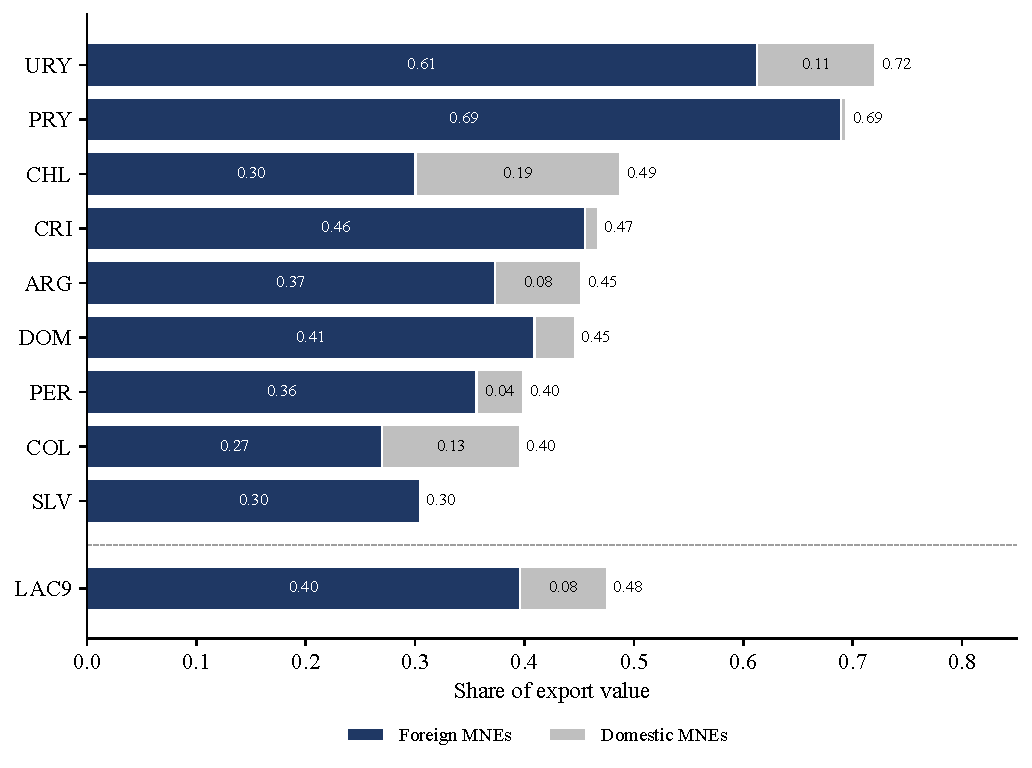
\includegraphics[width=0.72\textwidth,height=0.30\textheight,keepaspectratio]{figures/agro2018/fig_agp_origin_lac9.pdf}
\par\vspace{3pt}
{\small\textit{Panel B. Multinationals by parent country}}\par\vspace{1pt}
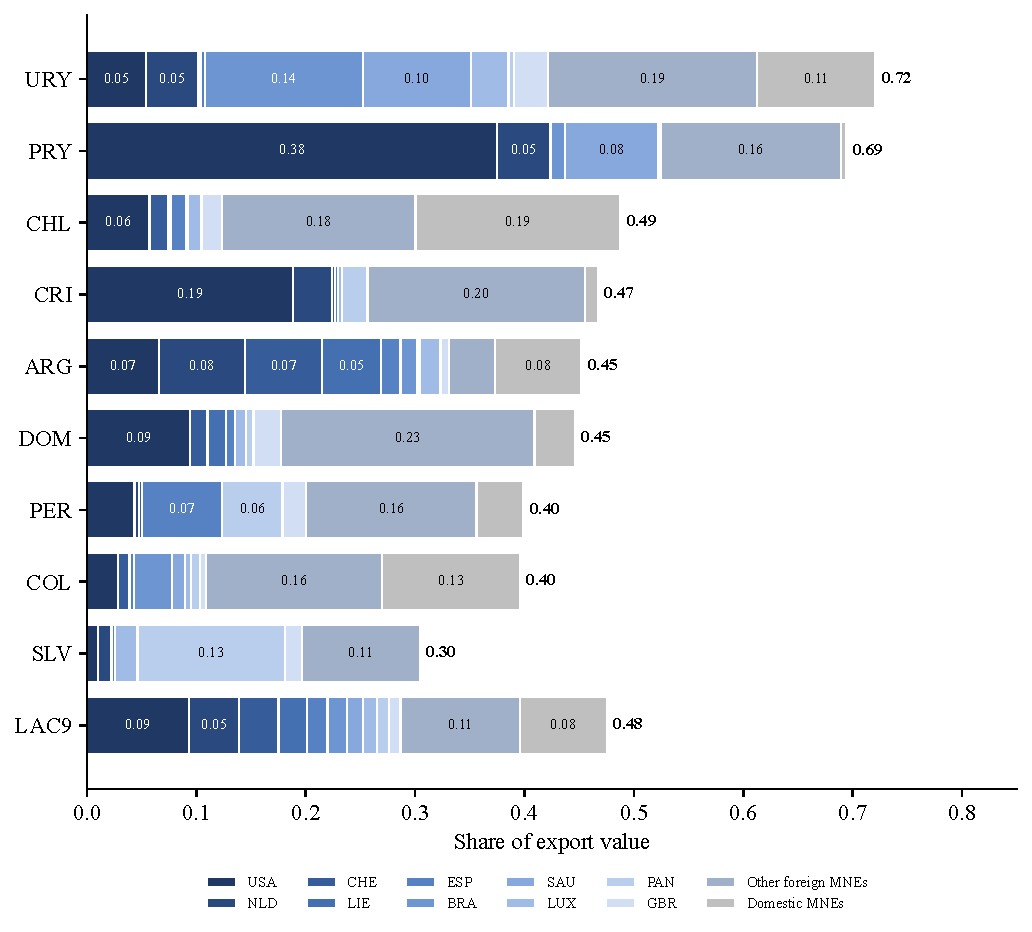
\includegraphics[width=0.85\textwidth,height=0.32\textheight,keepaspectratio]{figures/agro2018/fig_wp1a_origin_by_parent_lac9.pdf}

\begin{minipage}{0.9\linewidth}
\notesize
\vspace{0.6em}
\textit{Notes:} Shares of agricultural export value (HS chapters 01 to 24) in 2018. LAC9: the nine countries together. Panel A: the number at the end of each bar is the total MNE share. Panel B: the foreign share split among the ten largest parent countries and all other foreign parents, which include matched firms with no recorded parent country. Domestic MNEs have their parent in the exporting country.\\
\srcnote
\end{minipage}
\end{figure}

% ---- Table: Agricultural exporters and multinational affiliates, by exporting country, 2018
\begin{table}[htbp]
\centering
\caption{Agricultural exporters and multinational affiliates, by exporting country, 2018}
\label{tab:country}
{\footnotesize\setlength{\tabcolsep}{3pt}\setlength{\extrarowheight}{1pt}
\adjustbox{max width=\linewidth}{\begin{tabular}{lrrrll}
\toprule
Country & Exports (US\$ billion) & Exporters & MNE affiliates & Main parent country (\%) & Main destination (\%) \\
\midrule
Argentina & 34.6 & 2,879 & 901 & NLD (21) & BRA (9) \\
Peru & 10.0 & 2,538 & 455 & ESP (21) & USA (23) \\
Chile & 8.5 & 1,542 & 643 & JPN (22) & USA (24) \\
Colombia & 7.2 & 2,421 & 545 & DEU (22) & USA (39) \\
Paraguay & 6.6 & 358 & 111 & USA (54) & ARG (54) \\
Costa Rica & 4.8 & 1,123 & 170 & USA (41) & USA (32) \\
Uruguay & 3.5 & 357 & 124 & BRA (24) & CHN (36) \\
Dominican Republic & 2.2 & 1,342 & 179 & HKG (25) & USA (48) \\
El Salvador & 1.1 & 433 & 53 & PAN (44) & GTM (22) \\
\bottomrule
\end{tabular}
}}

\begin{minipage}{0.95\linewidth}
\notesize
\vspace{0.6em}
\textit{Notes:} Agricultural exports (HS chapters 01 to 24) in 2018. MNE affiliates: exporters linked to Orbis or Dun \& Bradstreet. Main parent country: the parent country with the largest share of the exports of foreign MNEs of the country with a recorded parent, and that share in percent. Main destination: the largest destination and its share of the agricultural exports of the country in percent.\\
\srcnote
\end{minipage}
\end{table}

The association between multinational presence and exports holds in every country (Table~\ref{tab:country_reg}). The
regression is equation~(\ref{eq:presence}) estimated country by country with destination $\times$ product and
destination $\times$ year fixed effects, the same comparison as column 4 of Table~\ref{tab:t1}. The elasticity of total
exports with respect to the number of multinationals ranges from 0.60 in Costa Rica to 1.01 in Uruguay, and the
coefficient on the presence of at least one multinational is positive and significant in every country. For local
firms, the elasticity is positive and significant in seven countries, from 0.24 in Colombia to 0.74 in Paraguay. It is
not significant in Costa Rica, where it is close to zero, and in El Salvador.

% ---- Table: Multinational presence and agricultural exports, by exporting country
\begin{table}[htbp]
\centering
\caption{Multinational presence and agricultural exports, by exporting country}
\label{tab:country_reg}
{\footnotesize\setlength{\tabcolsep}{4pt}\setlength{\extrarowheight}{1pt}
\adjustbox{max width=\linewidth}{\begin{tabular}{lccccr}
\toprule
 & \multicolumn{2}{c}{$\ln$ exports, all firms} & \multicolumn{2}{c}{$\ln$ exports, local firms} & \\
\cmidrule(lr){2-3}\cmidrule(lr){4-5}
 & $\ln$(number & At least & $\ln$(number & At least & Observations \\
 & of MNEs) & one MNE & of MNEs) & one MNE & (all firms, (2)) \\
 & (1) & (2) & (3) & (4) & \\
\midrule
Argentina & 0.858*** & 0.659*** & 0.450*** & 0.342*** & 36,380 \\
 & (0.041) & (0.033) & (0.050) & (0.029) &  \\
Peru & 0.937*** & 0.855*** & 0.553*** & 0.330*** & 27,550 \\
 & (0.053) & (0.060) & (0.061) & (0.047) &  \\
Chile & 0.733*** & 0.425*** & 0.290*** & 0.070** & 28,288 \\
 & (0.031) & (0.036) & (0.046) & (0.034) &  \\
Colombia & 0.724*** & 0.606*** & 0.242*** & 0.284*** & 21,975 \\
 & (0.055) & (0.068) & (0.063) & (0.052) &  \\
Paraguay & 0.863*** & 0.600*** & 0.737*** & 0.322*** & 4,679 \\
 & (0.095) & (0.102) & (0.138) & (0.079) &  \\
Costa Rica & 0.597*** & 0.566*** & -0.002 & -0.015 & 17,379 \\
 & (0.099) & (0.097) & (0.174) & (0.086) &  \\
Uruguay & 1.009*** & 0.528*** & 0.463*** & 0.192* & 7,375 \\
 & (0.097) & (0.104) & (0.153) & (0.109) &  \\
Dominican Republic & 0.608*** & 0.852*** & 0.290*** & 0.264*** & 23,798 \\
 & (0.067) & (0.095) & (0.076) & (0.072) &  \\
El Salvador & 0.661*** & 0.333** & 0.133 & 0.083 & 8,423 \\
 & (0.135) & (0.148) & (0.132) & (0.077) &  \\
\midrule
Destination $\times$ product FE & $\checkmark$ & $\checkmark$ & $\checkmark$ & $\checkmark$ & \\
Destination $\times$ year FE & $\checkmark$ & $\checkmark$ & $\checkmark$ & $\checkmark$ & \\
\bottomrule
\end{tabular}
}}

\begin{minipage}{0.95\linewidth}
\notesize
\vspace{0.6em}
\textit{Notes:} Regression at the level of destination country, product and year for each exporting country. Agricultural products, 2012 to 2018. Destination $\times$ product and destination $\times$ year fixed effects. The workbook also reports, for each country, the other four specifications of the progression. Columns 1 and 3: $\ln$ number of MNEs, observations with at least one MNE. Columns 2 and 4: indicator for at least one MNE, all observations. Standard errors clustered by destination country in parentheses. *** $p<0.01$, ** $p<0.05$, * $p<0.1$.\\
\srcnote
\end{minipage}
\end{table}

\FloatBarrier
\section{Conclusions}\label{sec:conclusions}

Multinational firms ship almost half of the agricultural exports of the nine countries, and their exports are
concentrated in a few parent countries and in a few large groups. Their weight varies widely across countries, from
30 percent in El Salvador to 72 percent in Uruguay. Where more multinationals export a product to a destination,
exports are larger, and so are the exports of local firms, mostly through a larger number of local exporters. The
exports of multinationals do not fall less with distance than those of local firms once each firm is compared across
destinations.

Two features of these patterns are specific to agriculture. First, both the weight of multinationals and their
association with exports are larger in field crops and in farm products made with more capital per worker. These are
the segments in which production is large and mechanized and exports move in bulk through storage, crushing and port
facilities. Both are smaller in horticultural and plantation crops, which use more labor and are grown by many smaller
farms. Second, capital intensity makes a difference at the farm stage but not at the processing stage. Among processed
products, multinationals ship similar shares, and their presence shows similar associations with exports, whether the
industry uses more or less capital per worker. The differences across products therefore line up with how the raw
product is grown rather than with how it is processed.

All these patterns are associations. They describe where multinationals and larger exports go together, not the
effect of multinational presence on exports. Measuring that effect would require changes in multinational presence
that are not related to the conditions of each market.

\section*{References}

\begin{list}{}{\leftmargin=1.5em \itemindent=-1.5em \itemsep=2pt \topsep=4pt}
\item Becker, R.\ A., Gray, W.\ B.\ and Marvakov, J., 2021. NBER-CES Manufacturing Industry Database (1958--2018, version 2021a). Cambridge, MA: National Bureau of Economic Research.
\item Clapp, J., 2015. ABCD and Beyond: From Grain Merchants to Agricultural Value Chain Managers. \emph{Canadian Food Studies}, 2(2), 126--135.
\item FAO, 2015. \emph{World Programme for the Census of Agriculture 2020, Volume 1: Programme, Concepts and Definitions}. FAO Statistical Development Series 15. Rome: Food and Agriculture Organization of the United Nations.
\item Kandel, W., 2008. Hired Farmworkers a Major Input for Some U.S. Farm Sectors. \emph{Amber Waves}, April 2008. Washington, DC: US Department of Agriculture, Economic Research Service.
\item Murphy, S., Burch, D.\ and Clapp, J., 2012. \emph{Cereal Secrets: The World's Largest Grain Traders and Global Agriculture}. Oxfam Research Reports. Oxford: Oxfam International.
\item Reardon, T., Barrett, C.\ B., Berdegu\'e, J.\ A.\ and Swinnen, J.\ F.\ M., 2009. Agrifood Industry Transformation and Small Farmers in Developing Countries. \emph{World Development}, 37(11), 1717--1727.
\item UNCTAD, 2009. \emph{World Investment Report 2009: Transnational Corporations, Agricultural Production and Development}. New York and Geneva: United Nations.
\item USDA NASS, 2019. \emph{2017 Census of Agriculture: United States Summary and State Data}, Volume 1, Geographic Area Series, Part 51. Washington, DC: US Department of Agriculture, National Agricultural Statistics Service.
\end{list}

\clearpage
\appendix
\setcounter{table}{0}\renewcommand{\thetable}{A.\arabic{table}}
\section*{Appendix}

% ---- Table: Multinational presence and agricultural exports, by type of production: extensive margin
\begin{table}[htbp]
\centering
\caption{Multinational presence and agricultural exports, by type of production: extensive margin}
\label{tab:crop_ext}
{\footnotesize\setlength{\tabcolsep}{4pt}\setlength{\extrarowheight}{1pt}
\adjustbox{max width=\linewidth}{\begin{tabular}{l*{5}{c}}
\toprule
 & (1) & (2) & (3) & (4) & (5) \\
\midrule
\multicolumn{6}{l}{\textit{Panel A. Dependent variable: $\ln$ exports, all firms}} \\
At least one MNE $\times$ horticultural and plantation crops & 1.985*** & 1.990*** & 0.606*** & 0.609*** & 0.533*** \\
 & (0.080) & (0.079) & (0.034) & (0.034) & (0.047) \\
At least one MNE $\times$ field crops & 1.803*** & 1.809*** & 0.759*** & 0.767*** & 0.614*** \\
 & (0.093) & (0.093) & (0.045) & (0.046) & (0.085) \\
At least one MNE $\times$ livestock and fisheries & 1.568*** & 1.556*** & 0.695*** & 0.678*** & 0.585*** \\
 & (0.086) & (0.086) & (0.046) & (0.047) & (0.065) \\
At least one MNE $\times$ other processed food & 1.701*** & 1.703*** & 0.664*** & 0.646*** & 0.619*** \\
 & (0.089) & (0.088) & (0.056) & (0.053) & (0.067) \\
$p$ value: field crops = horticultural and plantation crops & 0.042 & 0.044 & 0.004 & 0.004 & 0.400 \\
Observations (Panel A) & 199,737 & 199,649 & 179,134 & 177,453 & 90,773 \\
$R^2$ & 0.395 & 0.403 & 0.870 & 0.879 & 0.946 \\
\midrule
\multicolumn{6}{l}{\textit{Panel B. Dependent variable: $\ln$ exports, local firms}} \\
At least one MNE $\times$ horticultural and plantation crops & 2.178*** & 2.185*** & 0.229*** & 0.212*** & 0.128*** \\
 & (0.089) & (0.087) & (0.032) & (0.030) & (0.049) \\
At least one MNE $\times$ field crops & 2.203*** & 2.203*** & 0.404*** & 0.393*** & 0.212** \\
 & (0.083) & (0.083) & (0.042) & (0.043) & (0.099) \\
At least one MNE $\times$ livestock and fisheries & 1.644*** & 1.636*** & 0.350*** & 0.300*** & 0.037 \\
 & (0.080) & (0.079) & (0.040) & (0.042) & (0.078) \\
At least one MNE $\times$ other processed food & 1.451*** & 1.452*** & 0.127*** & 0.090** & -0.011 \\
 & (0.092) & (0.092) & (0.045) & (0.042) & (0.060) \\
$p$ value: field crops = horticultural and plantation crops & 0.808 & 0.867 & 0.001 & 0.001 & 0.459 \\
Observations (Panel B) & 158,241 & 158,168 & 140,246 & 138,532 & 63,068 \\
$R^2$ & 0.423 & 0.433 & 0.866 & 0.876 & 0.947 \\
\midrule
Origin FE & $\checkmark$ &  &  &  &  \\
Destination FE & $\checkmark$ &  &  &  &  \\
Product FE & $\checkmark$ & $\checkmark$ &  &  &  \\
Year FE & $\checkmark$ &  & $\checkmark$ &  &  \\
Origin $\times$ year FE &  & $\checkmark$ &  &  &  \\
Destination $\times$ year FE &  & $\checkmark$ &  &  &  \\
Origin $\times$ destination $\times$ product FE &  &  & $\checkmark$ & $\checkmark$ & $\checkmark$ \\
Origin $\times$ destination $\times$ year FE &  &  &  & $\checkmark$ & $\checkmark$ \\
Origin $\times$ product $\times$ year FE &  &  &  &  & $\checkmark$ \\
Destination $\times$ product $\times$ year FE &  &  &  &  & $\checkmark$ \\
\bottomrule
\end{tabular}
}}

\begin{minipage}{0.95\linewidth}
\notesize
\vspace{0.6em}
\textit{Notes:} Regressions as in Table~\ref{tab:crop}, with the indicator for at least one MNE in place of $\ln$ number of MNEs. All observations. Standard errors clustered by pair of origin and destination countries in parentheses. *** $p<0.01$, ** $p<0.05$, * $p<0.1$.\\
\textit{Source:} Authors' calculations based on customs data matched to Orbis (Bureau van Dijk) and Dun \& Bradstreet. Crop groups from the FAO Indicative Crop Classification.
\end{minipage}
\end{table}

% ---- Table: Multinational presence and agricultural exports, by capital intensity: extensive margin
\begin{table}[htbp]
\centering
\caption{Multinational presence and agricultural exports, by capital intensity: extensive margin}
\label{tab:capital_ext}
{\footnotesize\setlength{\tabcolsep}{4pt}\setlength{\extrarowheight}{1pt}
\adjustbox{max width=\linewidth}{\begin{tabular}{l*{5}{c}}
\toprule
 & (1) & (2) & (3) & (4) & (5) \\
\midrule
\multicolumn{6}{l}{\textit{Panel A. Dependent variable: $\ln$ exports, all firms}} \\
At least one MNE $\times$ farm stage, high capital intensity & 2.178*** & 2.176*** & 0.781*** & 0.789*** & 0.624*** \\
 & (0.103) & (0.104) & (0.059) & (0.060) & (0.114) \\
At least one MNE $\times$ farm stage, low capital intensity & 2.284*** & 2.292*** & 0.704*** & 0.699*** & 0.558*** \\
 & (0.103) & (0.103) & (0.044) & (0.042) & (0.071) \\
At least one MNE $\times$ processing stage, high capital intensity & 1.693*** & 1.695*** & 0.633*** & 0.634*** & 0.606*** \\
 & (0.070) & (0.069) & (0.035) & (0.035) & (0.049) \\
At least one MNE $\times$ processing stage, low capital intensity & 1.571*** & 1.562*** & 0.592*** & 0.573*** & 0.466*** \\
 & (0.082) & (0.082) & (0.055) & (0.055) & (0.082) \\
At least one MNE $\times$ not classified & 1.513*** & 1.518*** & 0.637*** & 0.639*** & 0.452*** \\
 & (0.100) & (0.101) & (0.075) & (0.077) & (0.114) \\
$p$ value: farm stage, high = low & 0.343 & 0.302 & 0.263 & 0.187 & 0.640 \\
$p$ value: processing stage, high = low & 0.075 & 0.052 & 0.446 & 0.261 & 0.113 \\
Observations (Panel A) & 198,231 & 198,142 & 177,525 & 175,847 & 85,000 \\
$R^2$ & 0.398 & 0.406 & 0.871 & 0.879 & 0.947 \\
\midrule
\multicolumn{6}{l}{\textit{Panel B. Dependent variable: $\ln$ exports, local firms}} \\
At least one MNE $\times$ farm stage, high capital intensity & 2.383*** & 2.375*** & 0.505*** & 0.505*** & 0.267* \\
 & (0.096) & (0.096) & (0.060) & (0.062) & (0.139) \\
At least one MNE $\times$ farm stage, low capital intensity & 2.469*** & 2.482*** & 0.358*** & 0.340*** & 0.126 \\
 & (0.110) & (0.108) & (0.044) & (0.042) & (0.083) \\
At least one MNE $\times$ processing stage, high capital intensity & 1.786*** & 1.787*** & 0.181*** & 0.162*** & 0.111** \\
 & (0.064) & (0.063) & (0.028) & (0.027) & (0.046) \\
At least one MNE $\times$ processing stage, low capital intensity & 1.502*** & 1.496*** & 0.199*** & 0.148*** & -0.025 \\
 & (0.088) & (0.088) & (0.051) & (0.051) & (0.081) \\
At least one MNE $\times$ not classified & 1.718*** & 1.723*** & 0.186*** & 0.165** & 0.088 \\
 & (0.097) & (0.097) & (0.067) & (0.072) & (0.155) \\
$p$ value: farm stage, high = low & 0.452 & 0.346 & 0.042 & 0.024 & 0.415 \\
$p$ value: processing stage, high = low & 0.000 & 0.000 & 0.735 & 0.804 & 0.141 \\
Observations (Panel B) & 156,990 & 156,915 & 138,938 & 137,240 & 58,746 \\
$R^2$ & 0.426 & 0.436 & 0.867 & 0.876 & 0.948 \\
\midrule
Origin FE & $\checkmark$ &  &  &  &  \\
Destination FE & $\checkmark$ &  &  &  &  \\
Product FE & $\checkmark$ & $\checkmark$ &  &  &  \\
Year FE & $\checkmark$ &  & $\checkmark$ &  &  \\
Origin $\times$ year FE &  & $\checkmark$ &  &  &  \\
Destination $\times$ year FE &  & $\checkmark$ &  &  &  \\
Origin $\times$ destination $\times$ product FE &  &  & $\checkmark$ & $\checkmark$ & $\checkmark$ \\
Origin $\times$ destination $\times$ year FE &  &  &  & $\checkmark$ & $\checkmark$ \\
Origin $\times$ product $\times$ year FE &  &  &  &  & $\checkmark$ \\
Destination $\times$ product $\times$ year FE &  &  &  &  & $\checkmark$ \\
\bottomrule
\end{tabular}
}}

\begin{minipage}{0.95\linewidth}
\notesize
\vspace{0.6em}
\textit{Notes:} Regressions as in Table~\ref{tab:capital}, with the indicator for at least one MNE in place of $\ln$ number of MNEs. All observations. Standard errors clustered by pair of origin and destination countries in parentheses. *** $p<0.01$, ** $p<0.05$, * $p<0.1$.\\
\textit{Source:} Authors' calculations based on customs data matched to Orbis (Bureau van Dijk) and Dun \& Bradstreet, USDA NASS, and NBER and CES.
\end{minipage}
\end{table}

\end{document}
